%%
%% This is file `sample-acmsmall.tex',
%% generated with the docstrip utility.
%%
%% The original source files were:
%%
%% samples.dtx  (with options: `all,journal,bibtex,acmsmall')
%% 
%% IMPORTANT NOTICE:
%% 
%% For the copyright see the source file.
%% 
%% Any modified versions of this file must be renamed
%% with new filenames distinct from sample-acmsmall.tex.
%% 
%% For distribution of the original source see the terms
%% for copying and modification in the file samples.dtx.
%% 
%% This generated file may be distributed as long as the
%% original source files, as listed above, are part of the
%% same distribution. (The sources need not necessarily be
%% in the same archive or directory.)
%%
%%
%% Commands for TeXCount
%TC:macro \cite [option:text,text]
%TC:macro \citep [option:text,text]
%TC:macro \citet [option:text,text]
%TC:envir table 0 1
%TC:envir table* 0 1
%TC:envir tabular [ignore] word
%TC:envir displaymath 0 word
%TC:envir math 0 word
%TC:envir comment 0 0
%%
%%
%% The first command in your LaTeX source must be the \documentclass
%% command.
%%
%% For submission and review of your manuscript please change the
%% command to \documentclass[manuscript, screen, review]{acmart}.
%%
%% When submitting camera ready or to TAPS, please change the command
%% to \documentclass[sigconf]{acmart} or whichever template is required
%% for your publication.
%%
%%
\documentclass[acmsmall]{acmart}

%%
%% \BibTeX command to typeset BibTeX logo in the docs
\AtBeginDocument{%
  \providecommand\BibTeX{{%
    Bib\TeX}}}

%% Rights management information.  This information is sent to you
%% when you complete the rights form.  These commands have SAMPLE
%% values in them; it is your responsibility as an author to replace
%% the commands and values with those provided to you when you
%% complete the rights form.
\setcopyright{acmlicensed}
\copyrightyear{2024}
\acmYear{2024}
\acmDOI{XXXXXXX.XXXXXXX}


%%
%% These commands are for a JOURNAL article.
\acmJournal{JACM}
\acmVolume{37}
\acmNumber{4}
\acmArticle{111}
\acmMonth{8}

%%
%% Submission ID.
%% Use this when submitting an article to a sponsored event. You'll
%% receive a unique submission ID from the organizers
%% of the event, and this ID should be used as the parameter to this command.
%%\acmSubmissionID{123-A56-BU3}

%%
%% For managing citations, it is recommended to use bibliography
%% files in BibTeX format.
%%
%% You can then either use BibTeX with the ACM-Reference-Format style,
%% or BibLaTeX with the acmnumeric or acmauthoryear sytles, that include
%% support for advanced citation of software artefact from the
%% biblatex-software package, also separately available on CTAN.
%%
%% Look at the sample-*-biblatex.tex files for templates showcasing
%% the biblatex styles.
%%

%%
%% The majority of ACM publications use numbered citations and
%% references.  The command \citestyle{authoryear} switches to the
%% "author year" style.
%%
%% If you are preparing content for an event
%% sponsored by ACM SIGGRAPH, you must use the "author year" style of
%% citations and references.
%% Uncommenting
%% the next command will enable that style.
%%\citestyle{acmauthoryear}

% Language setting
% Replace `english' with e.g. `spanish' to change the document language
\usepackage[english]{babel}

% Useful packages
\usepackage{amsmath}
\usepackage{graphicx}
%\usepackage{amssymb}
\usepackage{array}
\usepackage{minted}

% Configuration for minted package
\setminted{
    style=colorful, % Set code style to colorful
    fontsize=\scriptsize,
    linenos, % Enable line numbers
    breaklines, % Enable line breaks
    breakanywhere, % Allow line breaks anywhere
    autogobble,
}
%\usepackage[colorlinks=true, allcolors=blue]{hyperref}

\newcommand\teo[1]{\textcolor{red}{teo: #1}}
\newcommand\help[1]{\textcolor{green}{Help Needed: #1}}
\newcommand\willow[1]{\textcolor{purple}{Willow: #1}}

%%
%% end of the preamble, start of the body of the document source.
\begin{document}


%%
%% The "title" command has an optional parameter,
%% allowing the author to define a "short title" to be used in page headers.
\title{Finch: A Datastructure-Driven Array Programming Language}

%%
%% The "author" command and its associated commands are used to define
%% the authors and their affiliations.
%% Of note is the shared affiliation of the first two authors, and the
%% "authornote" and "authornotemark" commands
%% used to denote shared contribution to the research.
\author{Willow Ahrens}
\affiliation{%
  \institution{MIT CSAIL}
  \city{Cambridge}
  \state{Massachusetts}
  \country{USA}}
\email{willow@csail.mit.edu}

\author{Teodoro Fields Collin}
\affiliation{%
  \institution{MIT CSAIL}
  \city{Cambridge}
  \state{Massachusetts}
  \country{USA}}
\email{teoc@mit.edu}

\author{Radha Patel}
\affiliation{%
  \institution{MIT CSAIL}
  \city{Cambridge}
  \state{Massachusetts}
  \country{USA}}
\email{rrpatel@mit.edu}

\author{Kyle Deeds}
\affiliation{%
  \institution{University of Washington}
  \city{Seattle}
  \state{Washington}
  \country{USA}}
\email{kdeeds@cs.washington.edu}

\author{Changwan Hong}
\affiliation{%
  \institution{MIT CSAIL}
  \city{Cambridge}
  \state{Massachusetts}
  \country{USA}}
\email{changwan@mit.edu}

\author{Saman Amarasinghe}
\affiliation{%
  \institution{MIT CSAIL}
  \city{Cambridge}
  \state{Massachusetts}
  \country{USA}}
\email{saman@csail.mit.edu}

%%
%% By default, the full list of authors will be used in the page
%% headers. Often, this list is too long, and will overlap
%% other information printed in the page headers. This command allows
%% the author to define a more concise list
%% of authors' names for this purpose.
\renewcommand{\shortauthors}{Ahrens et al.}

%%
%% The abstract is a short summary of the work to be presented in the
%% article.
\begin{abstract}
From FORTRAN to Numpy, arrays have revolutionized how we express computation.  Arrays are the highest-performing datastructure with a long history of investment and innovation, from hardware support to compiler technology.  However, arrays can only handle dense rectilinear integer grids. Real world arrays often contain underlying structure, such as sparsity, runs of repeated values, or symmetry. We describe a compiler, Finch, which adapts existing programs and interfaces to the structure and sparsity of the inputs. Finch enables programmers to capture complex, real-world data scenarios with the same productivity they expect from dense arrays. Our approach enables new loop optimizations across multiple domains, unifying techniques such as sparse tensors, databases, and lossless compression. 
\end{abstract}

%%
%% The code below is generated by the tool at http://dl.acm.org/ccs.cfm.
%% Please copy and paste the code instead of the example below.
%%
\begin{CCSXML}
<ccs2012>
 <concept>
  <concept_id>00000000.0000000.0000000</concept_id>
  <concept_desc>Do Not Use This Code, Generate the Correct Terms for Your Paper</concept_desc>
  <concept_significance>500</concept_significance>
 </concept>
 <concept>
  <concept_id>00000000.00000000.00000000</concept_id>
  <concept_desc>Do Not Use This Code, Generate the Correct Terms for Your Paper</concept_desc>
  <concept_significance>300</concept_significance>
 </concept>
 <concept>
  <concept_id>00000000.00000000.00000000</concept_id>
  <concept_desc>Do Not Use This Code, Generate the Correct Terms for Your Paper</concept_desc>
  <concept_significance>100</concept_significance>
 </concept>
 <concept>
  <concept_id>00000000.00000000.00000000</concept_id>
  <concept_desc>Do Not Use This Code, Generate the Correct Terms for Your Paper</concept_desc>
  <concept_significance>100</concept_significance>
 </concept>
</ccs2012>
\end{CCSXML}

\ccsdesc[500]{Do Not Use This Code~Generate the Correct Terms for Your Paper}
\ccsdesc[300]{Do Not Use This Code~Generate the Correct Terms for Your Paper}
\ccsdesc{Do Not Use This Code~Generate the Correct Terms for Your Paper}
\ccsdesc[100]{Do Not Use This Code~Generate the Correct Terms for Your Paper}

%%
%% Keywords. The author(s) should pick words that accurately describe
%% the work being presented. Separate the keywords with commas.
\keywords{Do, Not, Us, This, Code, Put, the, Correct, Terms, for,
  Your, Paper}

\received{20 February 2007}
\received[revised]{12 March 2009}
\received[accepted]{5 June 2009}

%%
%% This command processes the author and affiliation and title
%% information and builds the first part of the formatted document.
\maketitle

\section{Introduction}

%Array programming is the core abstraction behind many of the modern miracles of computing (e.g. neural networks, scientific simulation, database processing). 
Arrays are the most fundamental abstraction in computer science. Arrays and lists are often the first-taught datastructure
\cite[Chapter 2.2]{abelson_structure_1996}, \cite[Chapter 2.2]{knuth_art_1997}.
%
Arrays are also universal across programming languages, from their introduction
in Fortran in 1957 to present-day languages like Python
\cite{backus_fortran_1957}, keeping more-or-less the same semantics.
%
Modern
array programming languages such as NumPy, SciPy, MatLab, TensorFlow, PyTorch,
and Halide have pushed the limits of productive data processing with arrays,
fueling breakthroughs in machine learning, scientific computing, image
processing, and more  \cite{harris_array_2020, virtanen_scipy_2020,
moler_history_2020, abadi_tensorflow_2016,
paszke_pytorch_2019,ragan-kelley_halide_2013}.
%
These frameworks have been the
subject of extensive industry investment to enable performant implementations,
and often operate at the peak capacity of the hardware they run on
\cite{lo_roofline_2015}.

The success and ubiquity of arrays is likely due to their simplicity. 
%
Since
their introduction, multidimensional arrays have represented dense, rectilinear,
integer grids of points. 
%
By \textbf{dense}, we mean that indices are mapped to value via a simple formula relating multidimensional space to linear memory.
%
This
simplicity enables extensive interoperability, convenience layers, and
optimizations by breaking the abstraction barrier between array representation
and array storage.  
%
Compilers understand dense array computations across many
programming constructs, such as for and while loops, breaks, parallelism,
caching, prefetching, multiple outputs, scatters, gathers, vectoriation,
loop-carry-dependencies, and more. Several optimizations have been developed for
dense arrays, such as loop fusion, loop tiling, loop unrolling, and loop
interchange.
%
However, while dense arrays are the easiest way to program, the world is not all dense.

%Bring in structure
% - old arrays are Dense, rectilinear, integer grids
% - The world is not like that
% - Sparsity, runs of repeated values, symmetry
% - Lots of citations, perhaps a few figures from my powerpoint
%Sparse arrays
% - Networks (graphblas, graph frameworks)
% - Simulations (BLAS, symblas, banded blas, etc)
% - Databases (database engines)
%Run-length encoding
%Symmetry
%Bands
%Padding
%Blocks
\help{This section needs citations, please help expand it and make it more
convincing. A figure could be nice.} 
\begin{figure}
	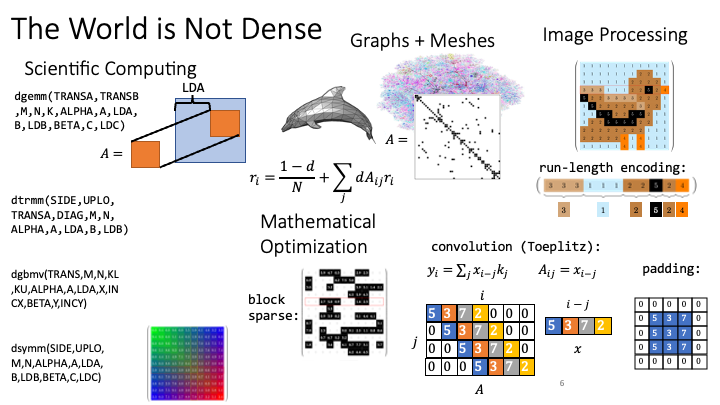
\includegraphics[width=\linewidth]{example_structures.png}
    \caption{some example structures that might be nice to put into a figure}
\end{figure}
Our world is full of structured arrays.
%

Sparse arrays (which store only nonzero elements) describe networks and
simulations.
%
Run-length encoding describes images and masks, geometry, and
databases (such as a list of transactions with the date field all the same)
Symmetry, bands, padding, and blocks are all natural matrix properties which
arise in the course of scientific computing or simulations of the natural world.
%

Operators, such as convolution, can be expressed as structured arrays.
%
For
example, a convolution with a filter can be expressed as a matrix multiplication
with the toeplitz matrix of all the circular shifts of the filter.

\help{This section needs citations}
\textbf{Currently, support for structured data is fragmented and incomplete}.
%
Experts must hand write variations of even the simplest kernels, like matrix
multiply, for each data structure and architecture to get performance.
%
Implementations must choose a small set of features to support well, resulting
in a compromise between \textbf{program flexibility} and \textbf{datastructure
flexibility}.
%
Hand-written solutions are collected in diverse libraries like
MKL, OpenCV, or SciPy. 
%
However, libraries will only ever support a subset of
programs on a subset of datastructure combinations. Even the most advanced
libraries, such as the GraphBLAS, which support a wide variety of sparse
operations over various semirings always lack support for other features, such
as tensors, fused outputs, or runs of repeated values. 
%
While dense array
compilers support an enormous variety of program constructs like early break and
multiple left hand sides, they only support dense arrays.  
%
Special-purpose
compilers like TACO or CoRa which support a select subset of structured data
structures (only sparse, or only ragged arrays) must compromise by greatly
constraining the classes of programs which they support, such as tensor
contractions \cite{kjolstad_tensor_2019, fegade_cora_2022}. 
%
This trade-off is
visualized in figure \ref{fig:datavsprogram}.

\begin{table}[h!]
  \help{This table needs citations, as well as a little bit of double checking}
  \centering
  \begin{tabular}{l|ccccc}
  \textbf{Feature / Tool} & \textbf{Halide} & \textbf{Taco} & \textbf{Cora} & \textbf{Taichi} & \textbf{Finch} \\
  \hline
  Einsums and Contractions & \checkmark & \checkmark & \checkmark & \checkmark & \checkmark \\
  High-Level API           &            & \checkmark &            &            & \checkmark \\
  Automatic API Fusion     &            &            &            &            & \checkmark \\
%  Parallelism              & \checkmark & \checkmark & \checkmark & \checkmark & \checkmark \\
  Multiple LHS             & \checkmark &            & \checkmark & \checkmark & \checkmark \\
  Affine Indices           & \checkmark &            &            & \checkmark & \checkmark \\
  Recurrence               & \checkmark &            &            &            &            \\
  If-Conditions and Masks  & \checkmark & \checkmark &            & \checkmark & \checkmark \\
  Scatter Gather           & \checkmark &            &            & \checkmark & \checkmark \\
  Early Break              &            & \checkmark &            &   \checkmark         & \checkmark \\
  \end{tabular}
  \caption{Feature support across various tools.}
  \label{tab:features}
  \end{table}
  
  \begin{table}[h!]
  \centering
  \begin{tabular}{l|ccccc}
  \textbf{Feature / Tool} & \textbf{Halide} & \textbf{Taco} & \textbf{Cora} & \textbf{Taichi} & \textbf{Finch} \\
  \hline
  Dense                    & \checkmark & \checkmark & \checkmark & \checkmark & \checkmark \\
  Padded                   & \checkmark &            &            &            & \checkmark \\
  One Sparse               &            & \checkmark &            & \checkmark & \checkmark \\
  Sparse                   &            & \checkmark &            &            & \checkmark \\
  Run-length               &            &            &            &            & \checkmark \\
  Symmetric                &            &            &            &            & \checkmark \\
  Regular Sparse Blocks    &            & \checkmark &            &            & \checkmark \\
  Irregular Sparse Blocks  &            &            &            &            & \checkmark \\
  Ragged                   &            &            & \checkmark &            & \checkmark \\
  \end{tabular}
  \caption{Support for various data structures across tools. Finch supports \textbf{both} complex programs and complex data structures.}
  \label{tab:data_structures}
\end{table}

We see two main challenges to writing efficient code over structured data.

\textbf{Optimizations are specific to the indirection and patterns in datastructures}: These structures break the simple mapping between array elements and where they are stored in memory. For example, sparse arrays store lists of which coordinates are nonzero, whereas run-length-encoded arrays map several pixels to the same color value. These zero regions or repeated regions are optimization opportunities, and we must adapt the program to avoid repetitive work on these regions by referencing the stored structure.

\textbf{Performance is highly structure dependent}: Structure aware kernels are dramatically faster than unstructured ones, and the landscape of implementation decisions is dramatically unpredictable. For example, sparse kernels don't need to compute on zeros, but this means that the precise input nonzero patterns act as computational filters, affecting the runtime as they interact with each other and the implementation.

In this work, we propose a new programming model we call ``Datastructure-driven Array Programming'' in which the programmer specifies the structure of the data separately from the program, and the compiler uses these two descriptions to generate efficient code. In this model, performance engineers can more efficiently search the
complex landscape of programs and datastructures to find the best implementation. In this programming model, we can express certain concepts in programs, and others in data. For example, if we wish to merge two sorted lists, we express this as two sparse vectors which are true whenever the list contains the key in question, and we iterate over the \textit{entire} space of keys, writing to the output list whenever either of the vectors are true.
While the order in which we iterate over the data is expressed in the program, which datapoints are of interest and how to find them is expressed in the data.

We develop a new array programming language, Finch, which supports \textit{both}
flexible programming constructs and diverse data structures. Finch supports a
familiar programming language of loops, statements, if conditions, breaks, etc,
over a wide variety of array structures, such as sparsity, run-length-encoding,
symmetry, triangles, padding, or blocks. The Finch compiler uses the structure
of the data to generate efficient implementations of these programs.

\subsection{Contributions}

\begin{enumerate}
\item More complex array structures than ever before. A complete level-by-level
structure-description language for expressing the structure of data
hierarchically. The first such set of formats to efficiently capture banded,
triangular, run-length-encoded, or sparse datasets, and any combination thereof.
\item A rich structured array programming language with for-loops
and complex control flow constructs at the same level of productivity
of dense arrays. To our knowledge, the Finch programming language is the first
to support if-conditions, early breaks, and multiple left hand sides over
structured data, as well as complex accesses such as affine indexing or scatter/gather.
\item A compiler that specializes programs to data structures 
predictably, facilitating an expressive language that makes it easier to search the complex
space of algorithms and datastructures. It is easy to implement new datastructures with a simple interface; the compiler analyzes the tensor lifecycle and inserts insert simple, overloadable, interface functions such as
initialization or finalization.
\item We evaluate the productivity of our language in several case studies,
showing that Finch can be used to accelerate a wide range of applications, 
from classic operations such as spmv and spgemm, to more complex applications such as image processing, graph analytics, and a high-level tensor operator fusion interface.
%We also demonstrate how Finch can fuse high-level operations to achieve a significant speedup over non-fused kernels. Additionally, as a case study, a high-level array programming language and fusion interface for operations such as map, broadcast, or reduce that can be compiled to efficient code using the previous loop-level abstractions.
%\item A complete set of level formats for expressing data patterns hierarchically in FiberTree-style decompositions. The first such set of formats to efficiently capture banded, triangular, run-length-encoded, or sparse-run-length-encoded datasets. The formats capture many use cases, from random updates to sequential construction.
%\item The Finch array language, mirroring simple for-loops with imperative code blocks and if-conditions. The first array programming language for the above data formats to support multiple outputs, affine indexing, and imperfectly-nested loops.
%\item Tensor lifecycles, a simple constraint on tensor reads and writes that elegantly restricts Finch programs to avoid complex data dependencies, and enables tensor polymorphism by providing implementers with well-defined functions to overload.
%\item Wrapper Tensors which modify existing datastructures and recombine them to support new patterns, such as affine indexing, padding, transposition, and slicing.
%\item Wrapper Levels which modify existing datastructures and enabling complex features such as atomic updates or contiguous versus separate allocation.
%\item We define the first mappings from the existing pydata/sparse array api high-level operations to low level finch notation
%\item <Performance Contributions>
\end{enumerate}


\section{Background}
\subsection{Looplets}
Finch represents iteration patterns using Looplets, a language that decomposes datastructure iterators hierarchically. Looplets represent the control-flow structures needed to iterate over any given datastructure, or multiple datastructures simultaneously. In particular, looplets are good at lifting code to the highest loop level that it's needed and subdividing iteration hierarchically in coordinate space. Because looplets are compiled with progressive lowering, structure-specific mathematical optimizations such as integrals, multiply by zero, etc. can be implemented using simple compiler passes like term rewriting and constant propagation.

We begin a formal description of looplets here:

\begin{figure}
	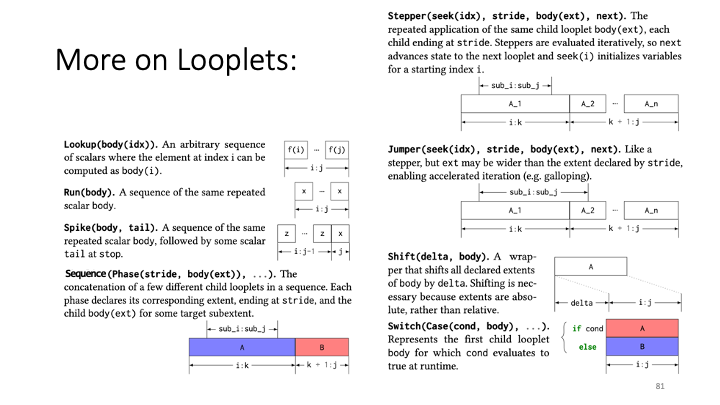
\includegraphics[width=\linewidth]{example_looplet_figure.png}
    \caption{Looplets visualized, along with their semantics}
\end{figure}

\subsection{FiberTrees}

\subsection{Concordant Iteration}

\subsection{Protocols}



\section{Bridging Looplets and Finch: The Tensor Interface}
\teo{I am doing stuff in this section.}
\section{Bridging Looplets and Finch: The Tensor Interface}

%
The Finch language provides descriptions of computations that iterate over a subset of a regular grid that is lexicographically ordered.
%
At this point, the reader might believe that compilation of a Finch program simply involves simply replacing for loops over a range with for loops over iterators, but Finch programs and data structures are sufficiently flexible that this impossible.
%
First, the Finch language interacts with multi-dimensional tensors whereas the Looplet abstraction is best suited towards iterators over a single dimension.
%
We require a bridge between the single dimensional iterators created from looplets and the mutli-dimensional abstractions common to tensor compilers.
%
Second, since the iteration order of a Finch program might not match that of a data structure (a discordant traversal), different iterators need to be requested for the same data depending on the traversal order of the program.
%
So we require a bridge that can provide different iteration orders depending on the context.
%
Third, since Finch programs can read and write to the same data, multi-dimensional tensors need to provide iterators for reading and writing as well as machinery to manage transition between these states.


To build our bridge, we embrace a set of abstractions: level formats/Fiber Trees, iteration context dependent instantiation of iterators, and tensor life cycles.
%
Our first abstraction mostly already exists in the literature: a manner of specifying a data structure for a multi-dimensional tensor out of data structures for single dimensional tensors~\cite{sze2017efficient,chou2022compilation, chou2018format}.
%
We recapitulate the essential details here.
%
Our next two abstractions add to to the first by providing a mechanism to use data structures generated by the first abstraction in a greater variety of contexts while maintaining per-dimension encapsulation of array data structures.
%
We introduce an interface to instatiate iterators in a variety of contexts in our programs and we introduce the lifecycle interface to manage when we read and write to multi-dimensional iterators.
%
These interfaces add to the level abstraction, expanding the types of data that they can express via mapping to looplets and expanding the contexts in which they can be used.
%
Previous efforts to compile a greater variety of sparse array programs left these bridges untouched ~\cite{henry_compilation_2021, won2023unified, senanayake2020sparse}.

%What needs to be said about the tensors? It's basically a few main points:
%1. (DONE) What is the level abstraction 
%2. (Done) We have identified 8 key level structures to represent most combinations of runs or pinpoints.
%2. a. beautiful figure with datas as rows of larger structures
%2. b. How do we write to each of these, in order? Randomly? random access? several important datastructures that show up along the way.
%3. What is "Unfurling"? and how does it help us represent each structure? refer to looplet decompositions of each case in the earlier figure
%4. What are lifecycles? How do lifecycles help us keep sane? Why are they necessary for correctness?

\subsection{Level Abstraction}
Fiber-tree style tensor abstractions have been the subject of extensive study
\cite{sze2017efficient, chou2022compilation, chou2018format}.  The underlying
idea is to represent a multi-dimensional tensor as a nested vector
datastructure, where each level of the nesting corresponds to a dimension of the
tensor. Thus, a matrix would be represented as a vector of vectors. This kind of
abstraction lends itself to representing sparse tensors if we vary the type of
vector used at each level in a tree. Thus, a sparse matrix might be represented
as a dense vector of sparse vectors. The vector of subtensors in this
abstraction is referred to as a \textbf{fiber}. Prior fiber-tree representations
focus on sparsity (where only the nonzero elements are represented) and treat
sparse vectors as sets of represented points. Since our fiber-tree
represesentation must handle other kinds of structure, such as diagonal,
repeated, or constant values, we instead view each fiber as a mapping from
indices into a space of subfibers.

%From the docs:
%Finch represents tensors hierarchically in a tree, where each node in the tree is a vector of subtensors and the leaves are the elements. Thus, a matrix is analogous to a vector of vectors, and a 3-tensor is analogous to a vector of vectors of vectors. The vectors at each level of the tensor all have the same structure, which can be selected by the user.
%In a Finch tensor tree, the child of each node is selected by an array index. All of the children at the same level will use the same format and share the same storage. Finch is column major, so in an expression A[i_1, ..., i_N], the rightmost dimension i_N corresponds to the root level of the tree, and the leftmost dimension i_1 corresponds to the leaf level.
%We refer to a node in the tree as a subfiber. All of the nodes at the same level are stored in the same datastructure, and disambiguated by an integer position. in the above example, there are three levels: the rootmost level contains only one subfiber, the root. The middle level has 3 subfibers, one for each column. The leafmost level has 12 subfibers, one for each element of the array. For example, the first level is A_fbr.lvl, and we can represent it's third position as SubFiber(A_fbr.lvl.lvl, 3). The second level is A_fbr.lvl.lvl, and we can access it's 9th position as SubFiber(A_fbr.lvl.lvl.lvl, 9). For instructional purposes, you can use parentheses to call a subfiber on an index to select among children of a subfiber.
%When we print the tree in text, positions are numbered from top to bottom. However, if we visualize our tree with the root at the top, positions range from left to right:
%Dense Format Index Tree
%Because our array is sparse, (mostly zero, or another fill value), it would be more efficient to store only the nonzero values. In Finch, each level is represented with a different format. A sparse level only stores non-fill values. This time, we'll use a tensor constructor with sl (for "SparseList of nonzeros") instead of d (for "Dense"):
%CSC Format Index Tree
%Our Dense(SparseList(Element(0.0))) format is also known as "CSC" and is equivalent to SparseMatrixCSC. The Tensor function will perform a zero-cost copy between Finch fibers and sparse matrices, when available. CSC is an excellent general-purpose representation when we expect most of the columns to have a few nonzeros. However, when most of the columns are entirely fill (a situation known as hypersparsity), it is better to compress the root level as well:
%DCSC Format Index Tree
%Here we see that the entirely zero column has also been compressed. The SparseList(SparseList(Element(0.0))) format is also known as "DCSC".
%The COO format is compact and straightforward, but doesn't support random access. For random access, one should use the SparseHash format. A full listing of supported formats is described after a rough description of shared common internals of level, relating to types and storage.
%All levels have a postype, typically denoted as Tp in the constructors, used for internal pointer types but accessible by the function:
%postype(lvl)

Instead of storing the data for each subfiber separately, most sparse tensor
formats such as CSR, DCSR, and COO usually store the data for all fibers in a
level contiguously. In this way, we can think of a level as a bulk allocator for
fibers. Continuing the analogy, we can think of each fiber as being
disambiguated by a \textbf{position}, or an index into the bulk pool of
subfibers. The mapping $f$ from indices to subfibers is thus a mapping from an
index and a position in a level to a subposition in a sublevel.
Figure~\ref{fig:levelsvsfibers} shows a simple example of a level as a pool of fibers.

When we need to refer to a particular fiber at position $p$ in the level $l$, we
may write $fiber(l, p)$. Note that the formation of fibers from levels is lazy,
and the data underlying each fiber is managed entirely by the level, so the
level may choose to overlap the storage between different fibers. Thus, the only
unique data associated with $fiber(l, p)$ is the position $p$.

\begin{figure}
    \centering
    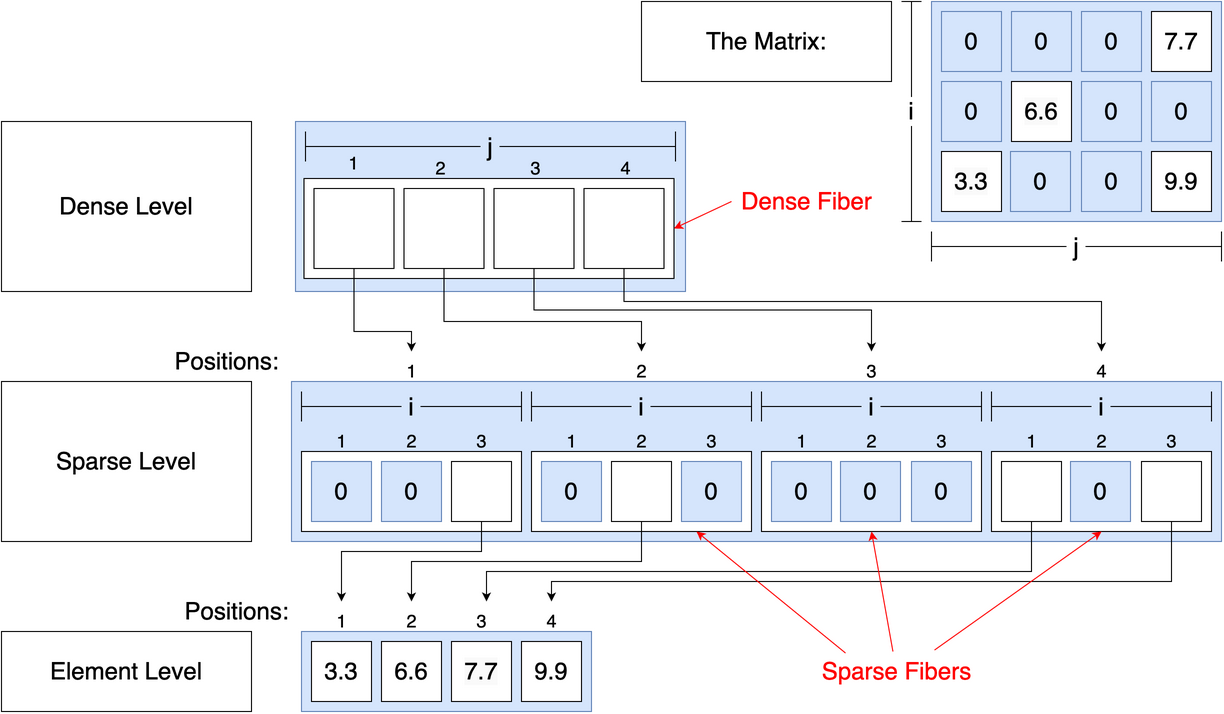
\includegraphics[width=0.45\linewidth]{LevelsVsFibers-matrix.png}\hfill%
    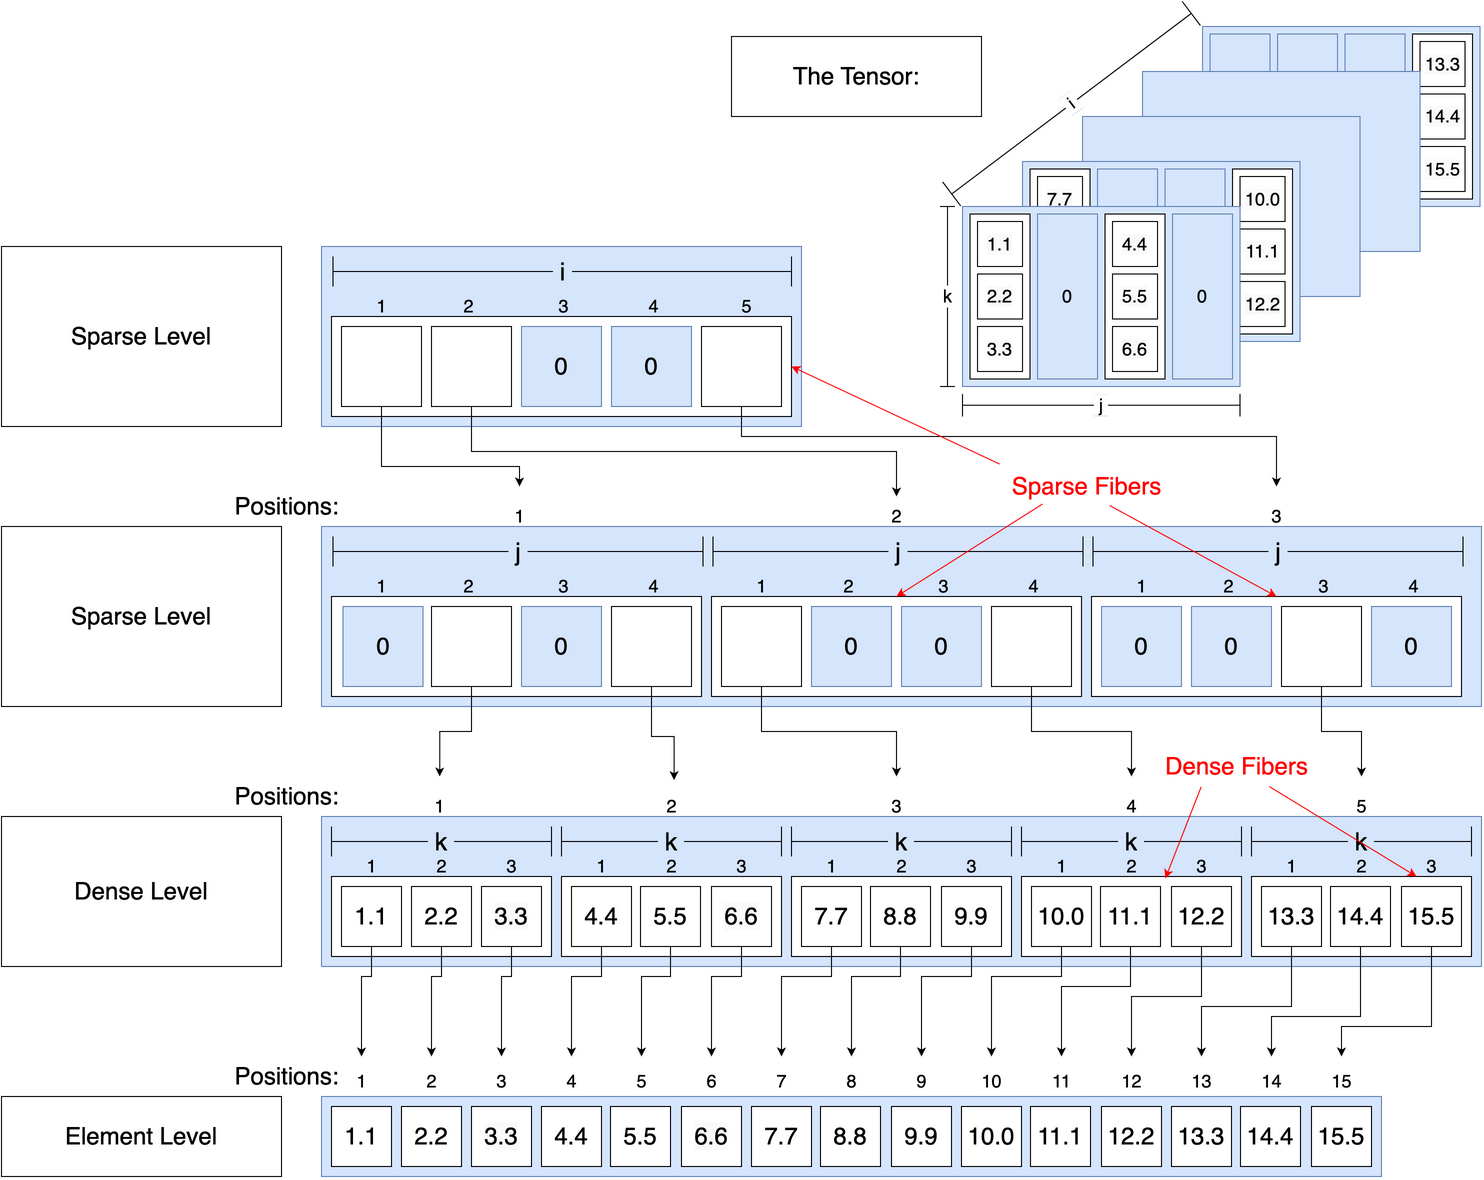
\includegraphics[width=0.5\linewidth]{LevelsVsFibers-tensor.png}
    \caption{Levels and fiber tree representations of a sparse matrix and a sparse tensor. On left, a matrix is represented in a fibertree corresponding to CSC format, with a dense outer level and a sparse inner level. On right, a tensor is represented in a fibertree with two sparse outer levels, and a dense inner level. Note that the element levels in this case form the leaves of the tree.}
    \label{fig:levelsvsfibers}
\end{figure}

\subsection{The 8 Key Level Structures}
    \begin{wrapfigure}{r}{.35\textwidth}
        \centering
        \scriptsize
        \begin{tabular}{|c|c|c|c|l|}
            \hline
            \rothead{Sparse} & \rothead{Blocked} & \rothead{Runs} & \rothead{Singletons} & \begin{tabular}{@{}l@{}}\textbf{Corresponding} \\ \textbf{Format}\end{tabular} \\
            \hline
             &  &  &  & Dense \\
            \hline
             &  & \checkmark &  & DenseRLE \\
            \hline
            \checkmark &  &  &  & Sparse \\
            \hline
            \checkmark &  &  & \checkmark & SparsePinpoint \\
            \hline
            \checkmark &  & \checkmark &  & SparseRLE \\
            \hline
            \checkmark &  & \checkmark & \checkmark & SparseInterval \\
            \hline
            \checkmark & \checkmark &  &  & SparseVBL \\
            \hline
            \checkmark & \checkmark &  & \checkmark & SparseBand \\
            \hline
        \end{tabular}
        \caption{All combinations of relevant structural properties and their
        corresponding formats.  Note that blocks and runs need not be considered
        together because we must store a run length for each run, and so there
        isn't a significant storage benefit to combining them. Blocks and
        singletons only make sense in the contex of sparsity, so we don't
        consider them together either. We omit such combinations
        from the exhaustive table.}
        \label{tab:TypesOfStructure}
    \end{wrapfigure}
    The main benefits of specializing to structure come from the following properties of the data:
    \begin{enumerate}
        \item[Sparsity] Sparse data is data that is mostly zero, or some other
        fill value. When we specialize on this data, we can use annihilation ($x
        * 0 = 0$), identity ($x * 1 = 1$), or other constant propagation
        properties ($ifelse(false, x, y) = y$) to simplify the computation and avoid
        redundant work.
        
        \item[Blocks] Blocked data is a subset of sparse data where the nonzeros
        are clustered and occur adjacent to one another. This provides us with
        two opportunities: We can avoid storing the locations of the nonzeros
        individually, and we can use more efficient randomly accessible
        iterators within the block. \cite{im_optimizing_2001, vuduc_performance_2002, ahrens_looplets_2023}.

        \item[Runs] Runs of repeated values may occur in dense or sparse code,
        cutting down on storage and allowing us to use integration rules such as 
        \mintinline{julia}{for i = 1:n; s += x end} $\rightarrow$
        \mintinline{julia}{s += n * x} or code motion to lift operations out of loops \cite{donenfeld_unified_2022,ahrens_looplets_2023}.

        \item[Singletons] When we have only one non-fill region in sparse data,
        we can avoid a loop entirely and reduce the complexity of iteration \cite{ghorbani2023compiling, ahrens_looplets_2023}.
    \end{enumerate}

    In Finch, we have identified 8 key level structures that can represent all
    of the relevant combinations of these properties, summarized in Table
    \ref{tab:TypesOfStructure}. We examine each structure in turn, describing
    some of the key properties and potential use cases of each. In this sense,
    the structures we consider are exhaustive. We can represent a wide variety
    of hierarchical tensor structures by combining these level structures in a
    tree, as shown in Figure~\ref{fig:structuraldiversity}.

    \begin{figure}
        \centering
        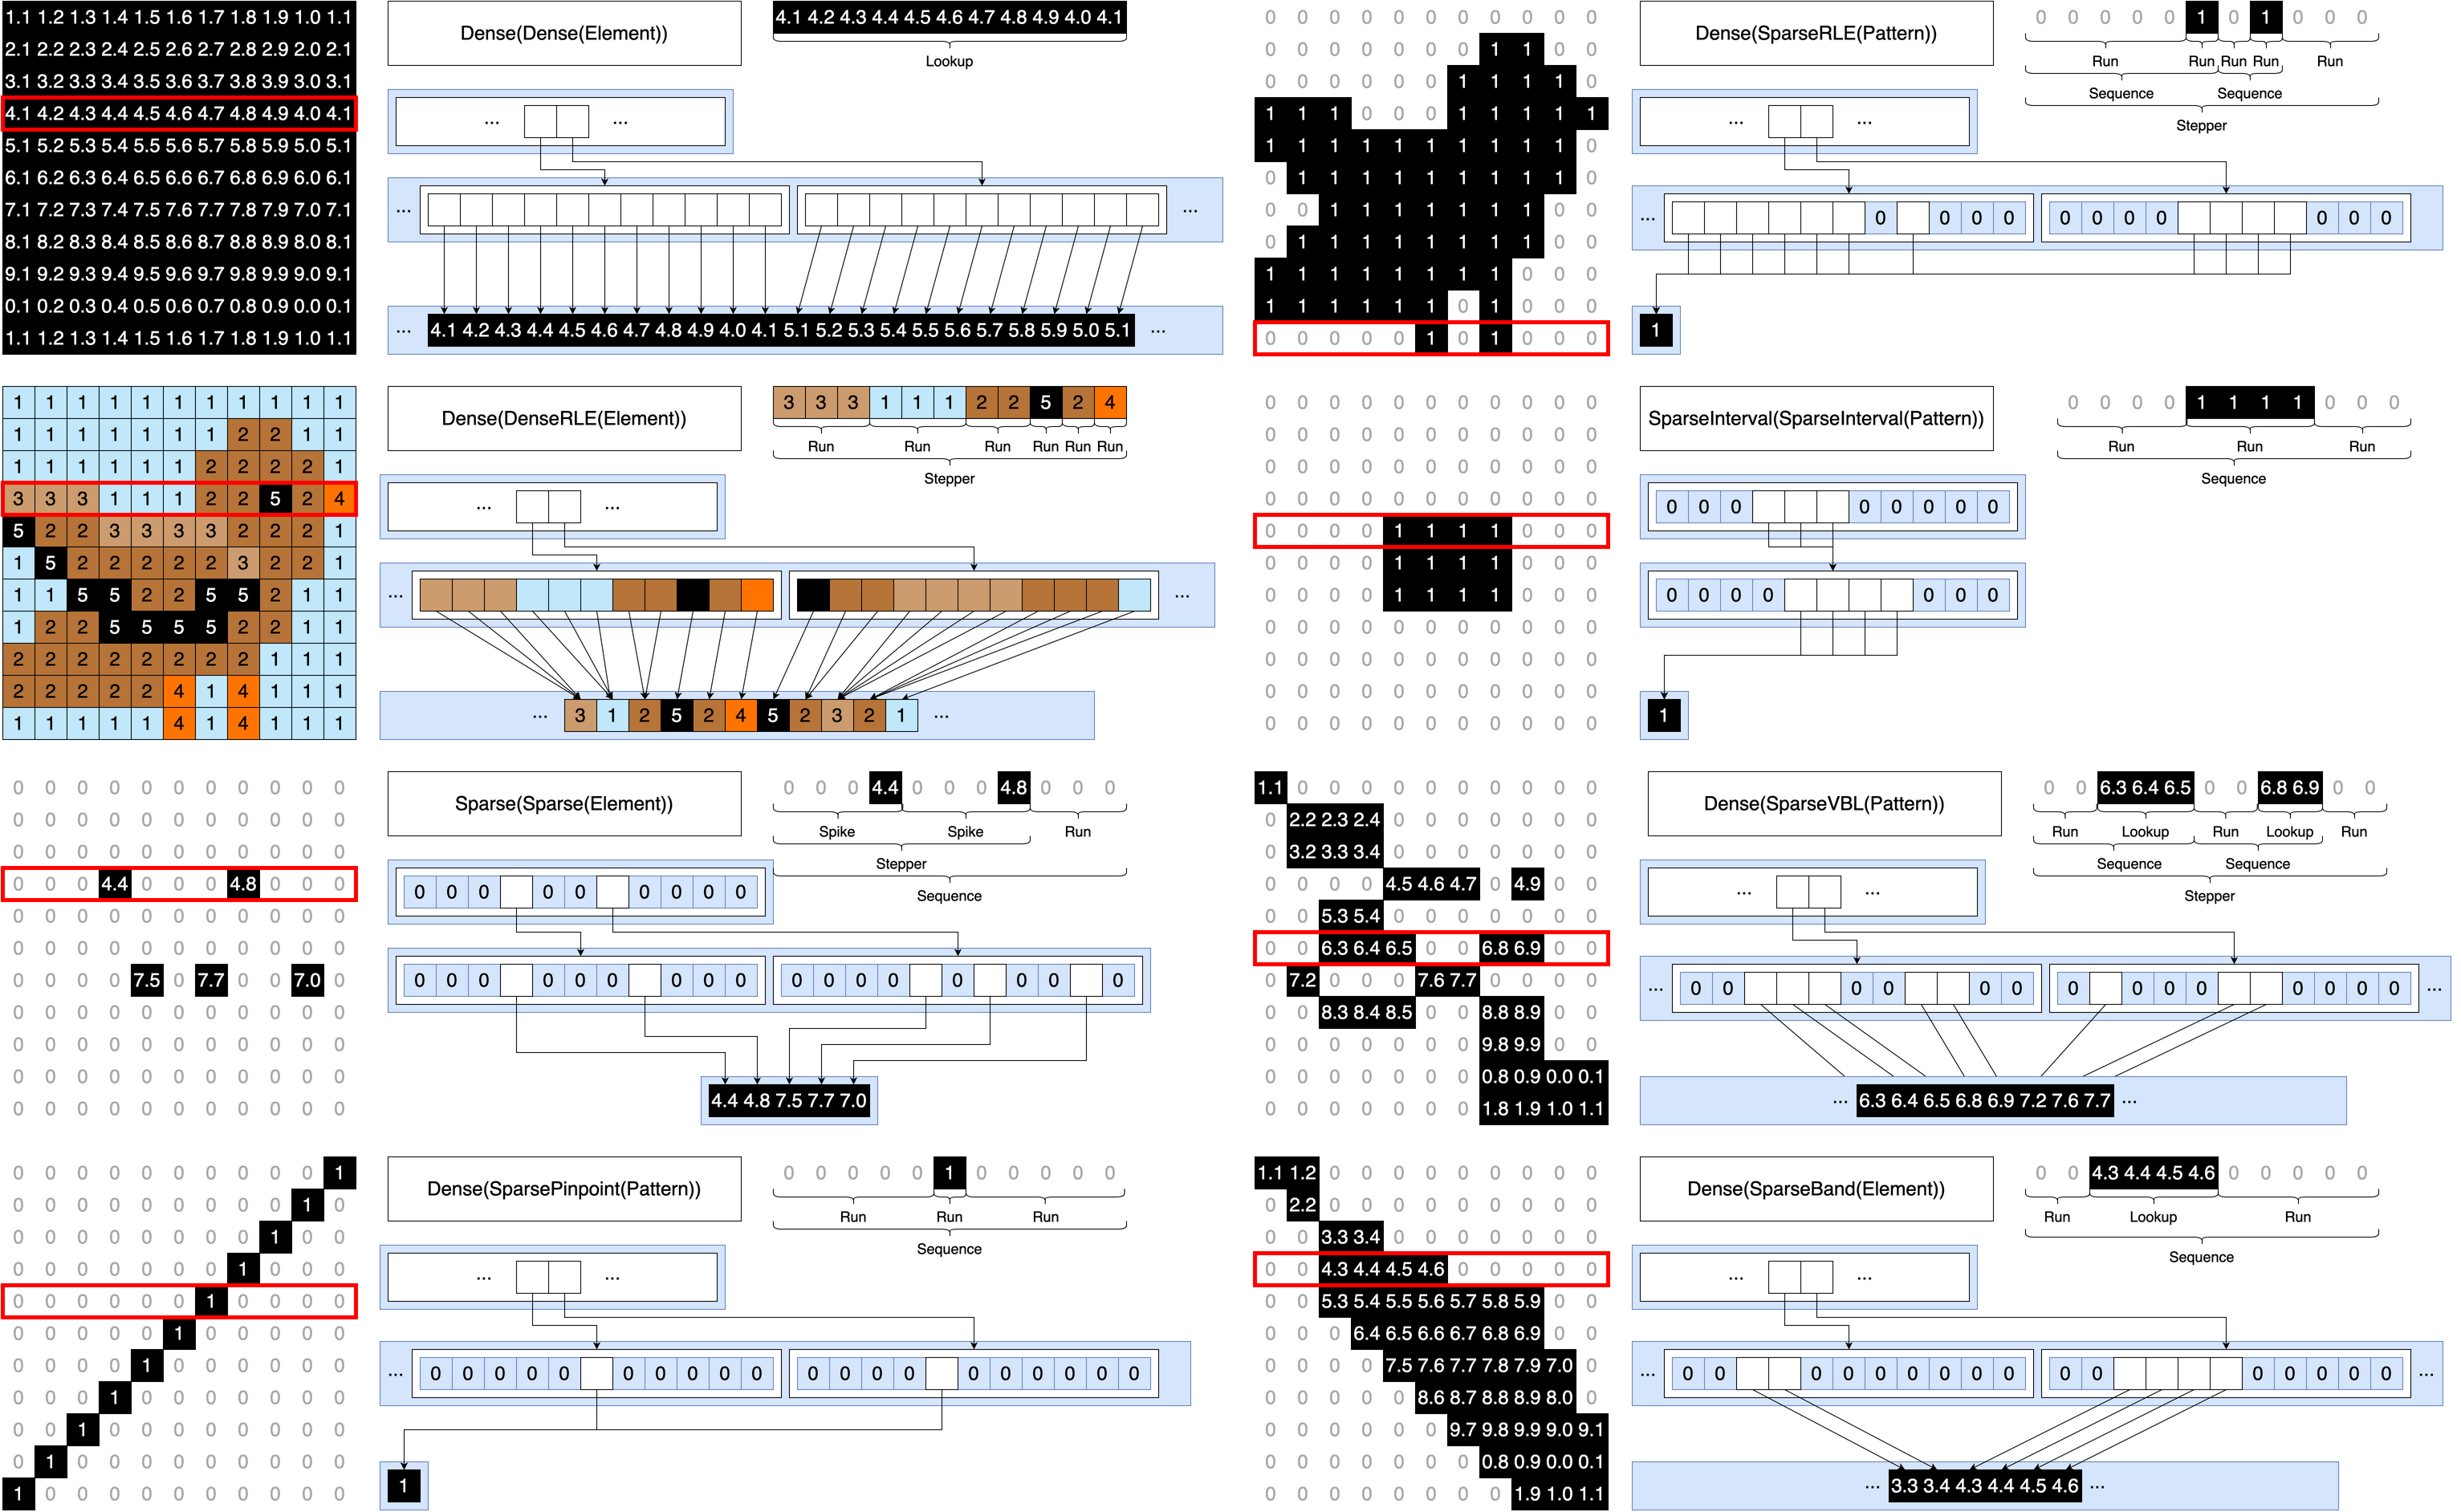
\includegraphics[width=\linewidth]{Structures.png}\hfill%
        \caption{Several examples of matrix structures represented using the
        level structures identified in Table~\ref{tab:TypesOfStructure}.
        Comparing this figure to \cite[Figure 3]{ahrens_looplets_2023}, we see
        that a level-by-level structural decomposition is diagrammed together
        with the Looplets.}
        \label{fig:structuraldiversity}
    \end{figure}

\subsection{Tensor Lifecycle, Declare, Freeze, Thaw, Unfurl}

Our simplified view of a level is enabled by our use of looplets to represent
the structure within each fiber. In fact, our level interface requires only 5
highly general operations, described below.

The first three of these functions, declare, freeze, and thaw, have to do with
managing when tensors can be assumed mutable or immutable. As we use Looplets to
represent iteration over a tensor, we must restrict the mutability of tensors
while we iterate over them. For example, if a tensor declares it has a constant
region from $i = 2:5$, but some other part of the computation modifies the
tensor at $i = 3$, this would result in incorrect behavior. It is much easier to
write correct Looplet code if we can assume that the tensor is immutable while
we are reading from it. Thus, we introduce the notion that a tensor can be in
read-only mode or update-only mode.  In read-only mode, the tensor may only
appear in the right-hand side of assignments. In update-only mode, the tensor
may only appear in the left-hand side of an assignment, either being overwritten
or incremented by some operator.  We can switch between these modes using freeze
and thaw functions. The declare function is used to allocate a tensor,
initialize it to some specified size and value, and leave it in update-only
mode. 

The unfurl function is used to manage iteration over a subfiber. At the point
when it comes time to iterate over a tensor, be in on the left or right hand
side of an assignment, we call the unfurl function to precompute whatever state
and datastructures are necessary to return a looplet nest that would iterate
over that level of a tensor. The unfurl function is called directly before
iterating over the corresponding loop, so it has access to any state variables introduced
by freezing or thawing the tensor.

Our view of a level as a fiber allocator implies an allocation function
$assemble(tns, pos_{start}:pos_{stop})$, which allocates fibers at positions
$pos_{start}:pos_{stop}$ in the level. We don't specify a de-allocation
function, instead relying on initialization to reset the fiber if it needs to be
reused. While all of the previous functions are used to manage the lifecycle and
iteration over a general tensor, the assemble function is quite specific to the
level abstraction, and the notion of positions within sublevels. Note: it was an
intentional choice to hold the parent level responsible for managing the
data of the sublevels, which positions they allocate, etc. This allows the parent
level to reuse allocation logic from internal index datastructures. For example,
a sparse level might use a list of indices to store which nonzeros are present,
and when it comes time to resize that list, it could also call assemble to resize the
sublevel, reducing the number of branches in the code. The assemble function
lends itself particularly to a "vector doubling" allocation approach, which we
have found to be effective and flexible when managing the allocation
of sparse left hand sides. This benefit is made clear in our evaluation section,
where we see that prior systems like TACO do not support all possible loop
orderings and format combinations for sparse matrix multiply because they do
not have a flexible enough allocation strategy, instead using a two-phase approach
which requires computing a complicated closed-form kernel to iterate over the
data twice to determine the number of required output nonzeros.

\begin{figure}
    \raggedright
\paragraph{$declare(lvl, init, dims...)$} Declares the level to hold subtensors
of size $dims$ and an initial value of $init$. Requires the level to be in
read-only mode.
\paragraph{$freeze(lvl)$} Finalizes the updates in the level, and readies the
level for reading. Requires the level to be in update-only mode.
\paragraph{$thaw(lvl)$} Prepares the level to accept updates. Requires the level
to be in read-only mode.
\paragraph{$unfurl(fiber(lvl, pos), ext, mode)$} Unfurls the fiber at position
$pos$ in the level $lvl$ over the extent $ext$. When $mode = \finchread$,
returns a looplet nest over the values in the read-only fiber.  When $mode =
\finchupdate$, returns a looplet nest over mutable subfibers in the update-only
fiber. Often, skipping over mutable locations allows the level to know which
locations must be stored. Additionally, a dirty bit may be used to communicate
whether the mutable subfiber has been written to, which allows the parent fiber
to know whether the subfiber must be stored explicitly.
\paragraph{$assemble(lvl, pos_{start}, pos_{stop})$} Allocates subfibers in the
level from positions $pos_{start}$ to $pos_{stop}$. Usually, this function is
only ever called on unassembled positions, but some levels (such as dense levels
or bytemaps) may support reassembly.
\caption{The five functions that define a level.}
\end{figure}

\subsection{Level Formats}
Having described the 8 basic level structures and the functions that define a
level format, we can describe the concrete level formats supported by Finch,
some of the challenges in their implementation, and how we overcome them. Note
that these formats are not meant to be exhaustive; we will later give
recommendations for additional level formats to be implemented and explain how
users can also add their own custom formats. Note that all of the levels below store their shape and a sublevel.

\begin{enumerate}
\item[Dense]
    The dense format is the simplest format, and simply maps $fiber(l, p)[i]
    \rightarrow fiber(l.lvl, p * l.shape + i)$. This format is used to store dense data,
    and is often a convenient format for the root level of a tensor. Because
    of its simplicity, freezing and thawing the level are no-ops.
\item[DenseRLE]
    The DenseRLE format is used to represent runs of repeated values. Notice
    that a challenge arises when trying to write to a level with runs: it is
    difficult to merge duplicate runs. Such a scenario might arise when merging
    runs of subfibers of length 3, representing colors in an image.  Ideally, we
    would be able to detect duplicate subfibers and merge them on the fly, but
    we cannot determine which subfibers are equal because we cannot read them
    while the sublevel is in update-only mode. Instead, we merge the duplicates
    during the freeze phase. We $freeze$ the main sublevel, $declare$ a separate
    sublevel as a buffer to store the deduplicated subfibers, and we can then
    compare each of the subfibers in the main level, copying the deduplicated
    subfibers into the buffer:
    \begin{enumerate}
        \item[$right$] A vector of indices corresponding to the end of each run in the level
        \item[$ptr$] A vector of delimiters such that $right[ptr[p]:ptr[p+1] - 1]$ is the set of delimiters in the subfiber at position $p$.
        \item[$buf$] A duplicate sublevel, used to store deduplicated subfibers during $freeze$.
    \end{enumerate}
\item[SparseList]
    The sparse list format is the simplest sparse format, and is used to
    construct the popular CSR, CSC, DCSR, DCSC, and CSF formats. The sparse list
    format consists of the following fields:
    \begin{enumerate}
        \item[$idx$] A vector of nonzero indices in the level
        \item[$ptr$] A vector of delimiters such that $idx[ptr[p]:ptr[p+1] - 1]$ is the set of nonzero indices in the subfiber at position $p$.
    \end{enumerate}
    All of Finch's sparse formats use a dirty bit during writing to determine
    whether the sublevel has been modified from it's default fill value and
    thus, whether it needs to be stored.
\item[SparsePinpoint]
    Because the SparsePinpoint format will only ever store one nonzero in each subfiber,
    we do not need the $ptr$ field.
    \begin{enumerate}
        \item[$idx$] A vector of nonzero indices in the level, one for each subfiber
    \end{enumerate}
\item[SparseRLE]
    Similar to the DenseRLE level, but because the runs are stored on top of a background of fill values, we must also store the start of each run.
    \begin{enumerate}
        \item[$left$] A vector of indices corresponding to the beginning of each run in the level
        \item[$right$] A vector of indices corresponding to the end of each run in the level
        \item[$ptr$] A vector of delimiters such that $left[ptr[p]:ptr[p+1] - 1]$ and $right[ptr[p]:ptr[p+1] - 1]$ are the set of delimiters in the subfiber at position $p$.
        \item[$buf$] A duplicate sublevel, used to store deduplicated subfibers during $freeze$.
    \end{enumerate}
\item[SparseInterval]
    Similar to the SparseRLE level, but $ptr$ is redundant because we only store
    one run. We also don't bother with deduplication here as we cannot store any
    intermediate results with duplicates.
    \begin{enumerate}
        \item[$left$] A vector of indices corresponding to the beginning of each run in the level
        \item[$right$] A vector of indices corresponding to the end of each run in the level
    \end{enumerate}
\item[SparseVBL]
    The SparseVBL format is used to represent blocked data. The format consists
    of the following fields:
    \begin{enumerate}
        \item[$idx$] A vector of indices at the end of each nonzero block in the level
        \item[$ptr$] A vector of delimiters such that $idx[ptr[p]:ptr[p+1] - 1]$ is the set of block terminals in the subfiber at position $p$.
        \item[$ofs$] A vector of delimiters such that $ofs[ptr[p] + q]:ofs[ptr[p] + q + 1] - 1$ are the subpositions of block $q$ in subfiber $p$.
    \end{enumerate}
\item[SparseBand]
    Like SparseVBL, but only one block is stored in each subfiber.
        \item[$idx$] The index at the end of the block in the level
        \item[$ofs$] A vector of delimiters such that $ofs[p]:ofs[p + 1] - 1$ are the subpositions of the block in subfiber $p$.
\end{enumerate}

\help{we need also to talk about pattern and element}

\subsection{Flexible Level Formats}
The levels we described in the previous section are all oriented towards bulk,
sequential creation of formats. However, when users want to be able to write out
of order (which is a common requirement arising from loop order or from the
problem itself, it occurs in our spgemm algorithms and our histogram example in
the evaluation section), we must use more complicated datastructures like hash
tables and trees to support the random access. Because these datastructures are
more complex and have a higher implementation burden and performance overhead,
we only support random access construction of sparse or dense structures.  We
can use these two more general structures as intermediates to convert to our
more specialized structures later.

\begin{enumerate}
\item[SparseHash]
    The sparse hash format uses a hash table to store the locations of nonzeros,
    and sorts the unique indices for iteration during the freeze phase. This
    allows for efficient random access, but not incremental construction, as the
    freeze phase runs in time proportional to the number of nonzeros in the
    entire level.
    \begin{enumerate}
        \item[$idx$] A vector of nonzero indices in the level
        \item[$ptr$] A vector of delimiters such that $idx[ptr[p]:ptr[p+1] - 1]$ is the set of nonzero indices in the subfiber at position $p$.
        \item[$tbl$] A hash table used for construction of the level.
    \end{enumerate}
\item[SparseBytemap]
    The SparseBytemap format uses a bytemap to store which locations have been
    written to. Unlike the SparseHash format, the bytemap assembles the entire
    space of possible subfibers. This accelerates random access in the format,
    but requires a high memory overhead. Because we don't want to reallocate all
    of the memory in each iteration, the declaration of this format instead
    re-assembles only the dirty locations in the tensor. This format is
    analogous to the default workspace format used by TACO.
    \begin{enumerate}
        \item[$idx$] A vector of nonzero indices in the level
        \item[$ptr$] A vector of delimiters such that $idx[ptr[p]:ptr[p+1] - 1]$ is the set of nonzero indices in the subfiber at position $p$.
        \item[$tbl$] A dense array of booleans used to mark dirty locations in the tensor.
    \end{enumerate}
\end{enumerate}

As future work, we also recommend the implementation of a tree-based format, as
this would enable incremental construction. Currently, the cost of freezing and
thawing is usually proportional to the number of stored fibers, so an operation
that sets a single value in a tensor would be prohibitively expensive (i.e.
$A[3, 4] = 3.14$). We would also recommend supporting SparseRLE as an
intermediate randomly accessible structure, because (unlike blocks or
singletons), runs have asymptotic benefits. However, these cases were not
necessary for our case studies.

\subsection{Scalars}

\subsubsection{Sparse Scalars}
\subsubsection{Early Break Scalars}



\subsection{Wrapper Tensors}

\subsection{Scalars}

\subsubsection{Sparse Scalars}
\subsubsection{Early Break Scalars}

\section{The Finch Language}

\subsection{Syntax and Semantics}

\section{The Finch Compiler}

\subsection{Dimensionalization}

\subsection{Concordization}

\subsection{Bounds Analysis}

\subsection{Performance Warnings}

\subsection{Wrapperization}

\subsection{Simplification and Algebraic Transformations}


\section{Evaluation}

\subsection{Data-Driven Performance Engineering}
\subsubsection{Sparse-Sparse Matrix Multiply}

\help{The main points of this section are:}

\help{1. summarize the difference between inner, gustavson, and outer, cite gamma but this also needs to stand on it's own}


\help{2. Explain why bytemap temporary makes sense for gustavson, but not for outer or inner}

\help{3. Point out that TACO does not even support outer product because it does not support scatter into 2D workspace}

\help{4. Take a look at the figure and point out that Finch is competitive with TACO on inner and gustavson, and that for outer product we see what we would expect from TACO: i.e. Finch Outer with dense performs similarly to TACO with dense, and Finch Outer with sparse performs much better as the matrix size increases.}

\help{5. point out that for the large matrices finch is competitive with TACO for gustavson}.

\help{6. explain the features of "datastructure-driven programming" that are used here in this problem. i.e. explicit temporary, bytemap format, transpositions}.
\begin{figure}
	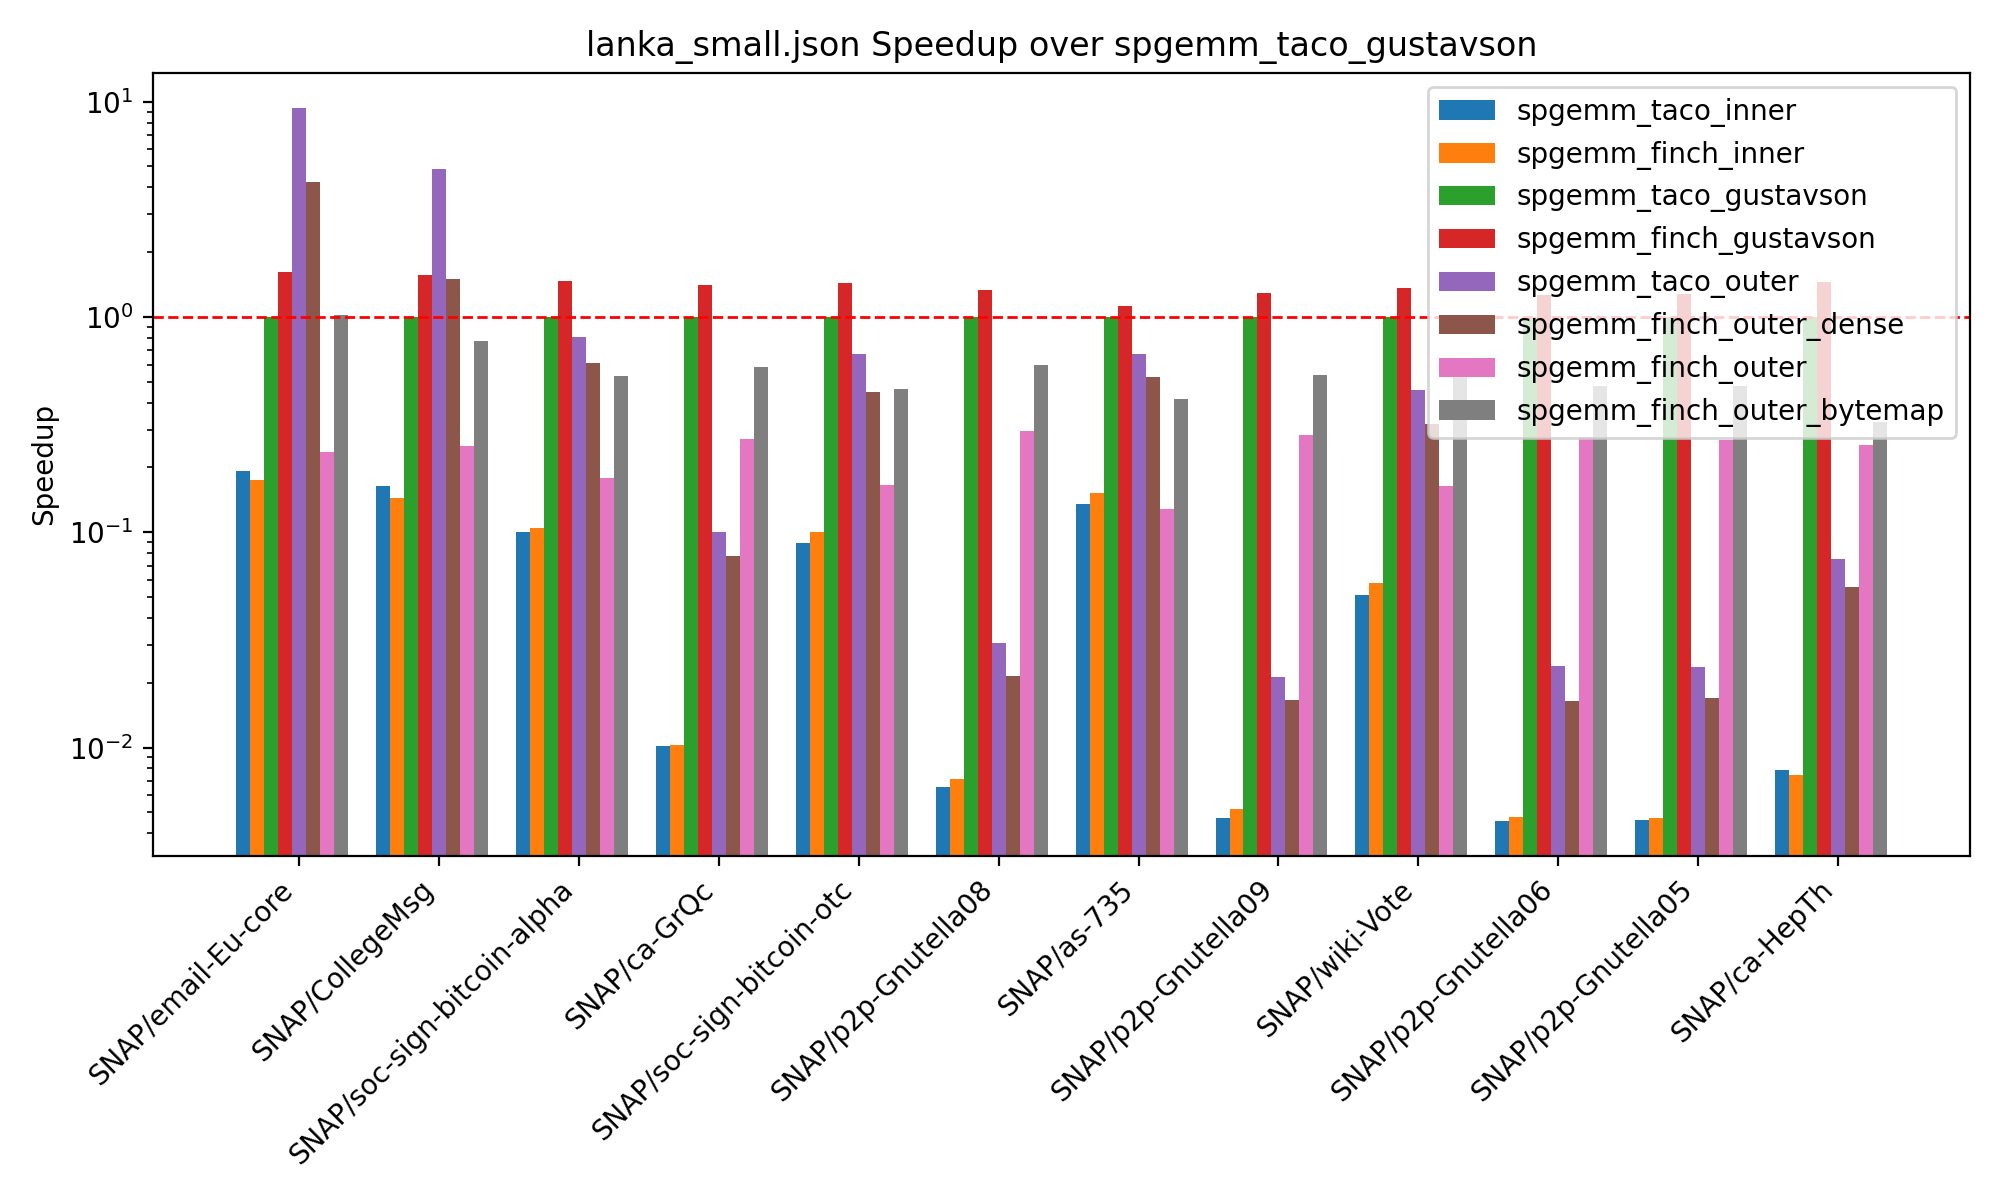
\includegraphics[width=\linewidth]{spgemm_small_speedup_log_scale.png}
    \caption{A comparison of several matrix multiplication algorithms between Finch and Taco smaller matrices, ordered from small to big dimension. Note that inner products necessarily requires $O(n^2)$ work and taco's outer products format is dense. Finch can use a sparse outer products format and thus has an asymptotic advantage that becomes evident as the output dimensions grow.}
\end{figure}

\begin{figure}
	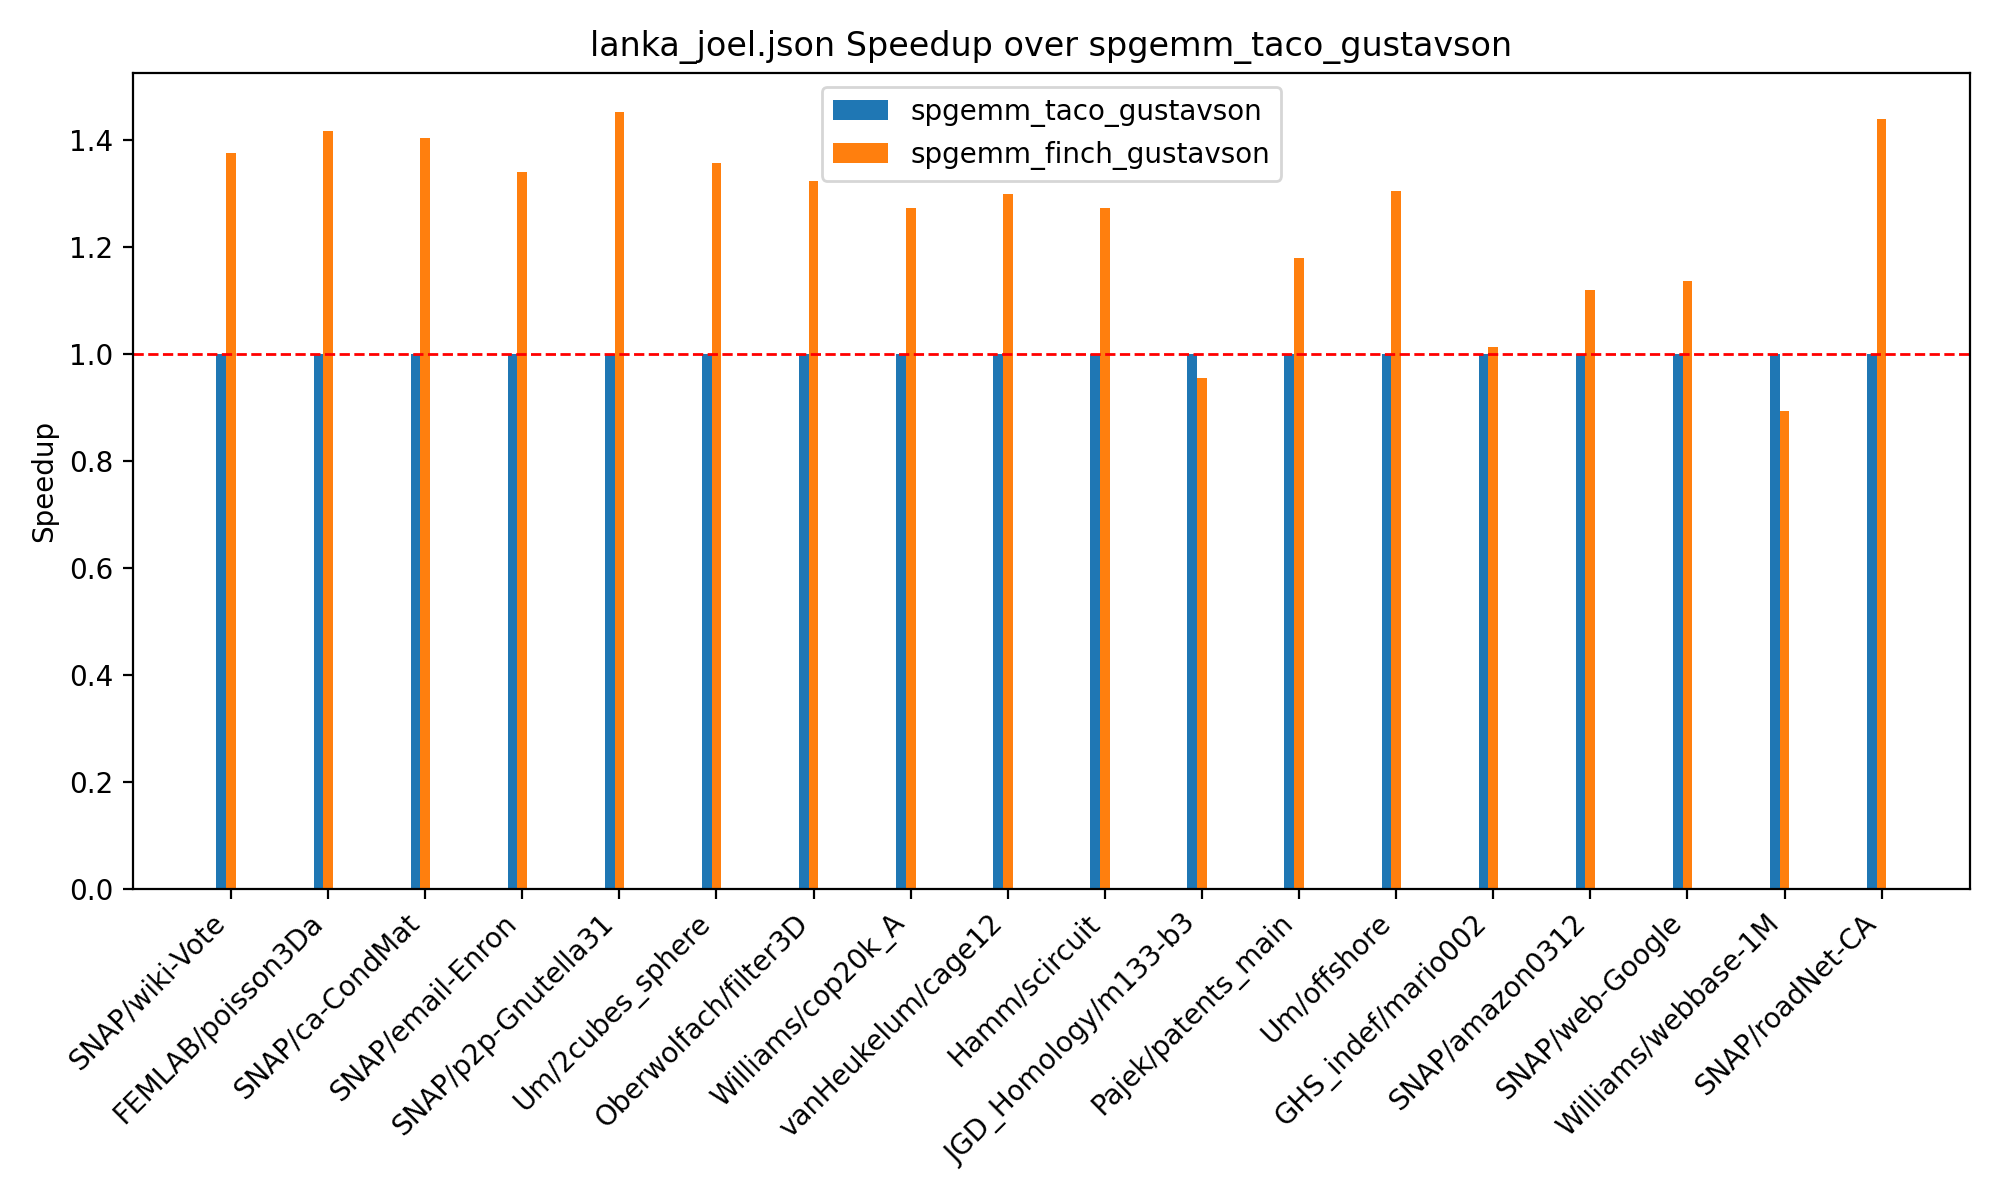
\includegraphics[width=\linewidth]{spgemm_joel_speedup.png}
    \caption{A comparison of gustavson's algorithm between Finch and Taco on some larger matrices}
\end{figure}

Examples that demonstrate performance engineering in a datastructure-driven model

\subsubsection{SpMV}
Finch provides many flexible level formats to efficiently capture a variety of patterns in datasets, encompassing both the structure and type of data. More specifically, these formats can represent banded, triangular, run-length-encoded, blocked, hashed, and boolean data, as well as several other formats. Finch also provides the control flow necessary to manipulate the order in which data in these flexible level formats is read and written, enabling us to take advantage of multiple structural patterns concurrently—for example, we can exploit both sparsity and symmetry by using a sparse level format and restricting data reads to one triangle of a matrix. % I'm not sure if the right place for this is here - maybe should come earlier?

Structure in data arises both naturally, due to the chemical and physical properties of matter, and artificially via mathematical operations that induce particular patterns. Closely tailoring a storage format to a particular data pattern enables us to reduce the amount of stored values, make data accesses more efficient, and take advantage of spatial locality, resulting in more performant code.

The sparse matrix-vector multiplication kernel is a common operation in sparse linear algebra with many applications including conjugate gradients, graph algorithms, numerical analysis, and neural networks. The wide range of applications unsurprisingly results in a wide range of types of datasets making it an effective kernel to demonstrate the utility of having flexible data formats. In this case study, we highlight a few different Finch formats and the performance effects of conforming a dataset’s structure with its storage format, which Finch's datastructure-driven model enables us to do.

We compare Finch’s performance to that of TACO, SuiteSparseGraphBLAS, and Julia’s standard library.  We test using sparse matrices from a large selection of datasets spanning several previous papers: the datasets used by Vuduc et al. to test the OSKI interface [cite], Ahrens et al. to test a variable block row format partitioning strategy [cite], and Kjolstad et al. to test the TACO library [cite]. In addition, we also created several synthetic matrices containing bands or blocks of varying sizes as well as a permutation matrix to encapsulate a few additional use cases. The dense vector is randomly generated. We depict the performance of SpMV across the aforementioned tools and compare to the fastest Finch format for that particular dataset in Figures 1 and 2. 

% TODO: make this be 3 columns
\begin{figure}
    \begin{minipage}[t]{0.315\textwidth}
        \vspace{0pt} % Add this to ensure top alignment within minipage
        \begin{minted}{julia}
            @finch begin
                y .= 0
                for j = _, i = _
                    y[i] += A[i, j] * x[j]
                end
                return y
            end
        \end{minted}
    \end{minipage}%
    \begin{minipage}[t]{0.315\textwidth}
        \vspace{0pt} % Add this to ensure top alignment within minipage
        \begin{minted}{julia}
            @finch begin
                y .= 0
                for j = _, i = _
                    y[j] += A[i, j] * x[i]
                end
                return y
            end
        \end{minted}
    \end{minipage}
    \begin{minipage}[t]{0.36\textwidth}
        \vspace{0pt} % Add this to ensure top alignment within minipage
        \begin{minted}{julia}
            @finch begin
                y .= 0
                for j = _
                    let x_j = x[j]
                        y_j .= 0
                        for i = _
                            let A_ij = A[i, j]
                                y[i] += x_j * A_ij
                                y_j[] += A_ij * x[i]
                            end
                        end
                        y[j] += y_j[] + diag[j] * x_j
                    end
                end
                return y
            end
        \end{minted}
    \end{minipage}
    \caption{Performance of SpMV across various tools.}
\end{figure}

\subsubsection{Tensor Formats}
We benchmarked the SpMV kernel using the Dense level format for the outer level and the SparseList, SparseVBL, SparseBand, and SparsePoint Finch levels for the inner level of the sparse matrix. To represent scalar values, we benchmarked with both the Element and Pattern levels. The SparseList, SparseVBL, and SparseBand formats were functional for all matrices, but the SparsePoint format was applicable only for the synthetic permutation matrices. The Element format was applicable to represent scalars in all matrices, while the Pattern level was applicable only for boolean matrices. 

We found that the SpMV performance was superior for the level format that best paralleled the structure of the tensor. Namely, matrices with a clear blocked structure like $exdata\_1$, $TSOPF\_RS\_b678\_c1$, and $heart3$ performed notably well with the SparseVBL format in comparison to both TACO and the Finch SparseList formats (which we consider the closest analog to the sparse matrix format used in TACO and other libraries) with speedups of 2.16, X, and Y relative to TACO and of 1.47, X, and Y relative to the SparseList Finch SpMV implementation. Furthermore, the synthetic Toeplitz banded matrices we constructed performed the best with the SparseBand matrix, in particular with the $toeplitz\_large\_band$ and the $toeplitz\_medium\_band$ matrices having a speedup of A and B relative to TACO and a speedup of A and B relative to the SparseList Finch SpMV implementation. 

There were also significant advantages of using the Pattern format instead of the Element format to represent scalar values in the matrices when these values were boolean. The matrices in the SNAP collection which represent graph datasets are boolean and had an average speedup of X over TACO and X over the same Finch program, but with an Element format.   


\subsubsection{Symmetric SpMV}
Finch enables us to exploit symmetry in the sparse matrix of the SpMV kernel by providing the capabilities to reuse memory reads and insert control flow logic to restrict iterations to either the lower or upper triangle of the sparse matrix. We can apply this strategy with any level format. Every symmetric matrix in the SparseList and SparseList-Pattern formats has better performance when we use a Finch SpMV program that takes advantage of this symmetry. However, the regular Finch SpMV program has better performance for symmetric matrices than the symmetric Finch SpMV program for the other more specialized formats, likely because we need in-order accesses to fully capitalize on the specialized storage. Symmetric SpMV with the SparseList level format in Finch results in an average of 1.3x speedup over TACO and symmetric SpMV with the SparseList-Pattern format in Finch results in an average speedup of 1.15x over TACO . Notably, there is a 1.9x speedup for the HB/saylr4 matrix. 
\subsubsection{4D Blocked SpMV}



%Here's a figure with spmv_performance_sorted_(faster_than_taco).png and spmv_performance_sorted_(slower_than_taco).png

\begin{figure}
    \begin{minipage}[t]{0.5\textwidth}
        \vspace{0pt} % Add this to ensure top alignment within minipage
        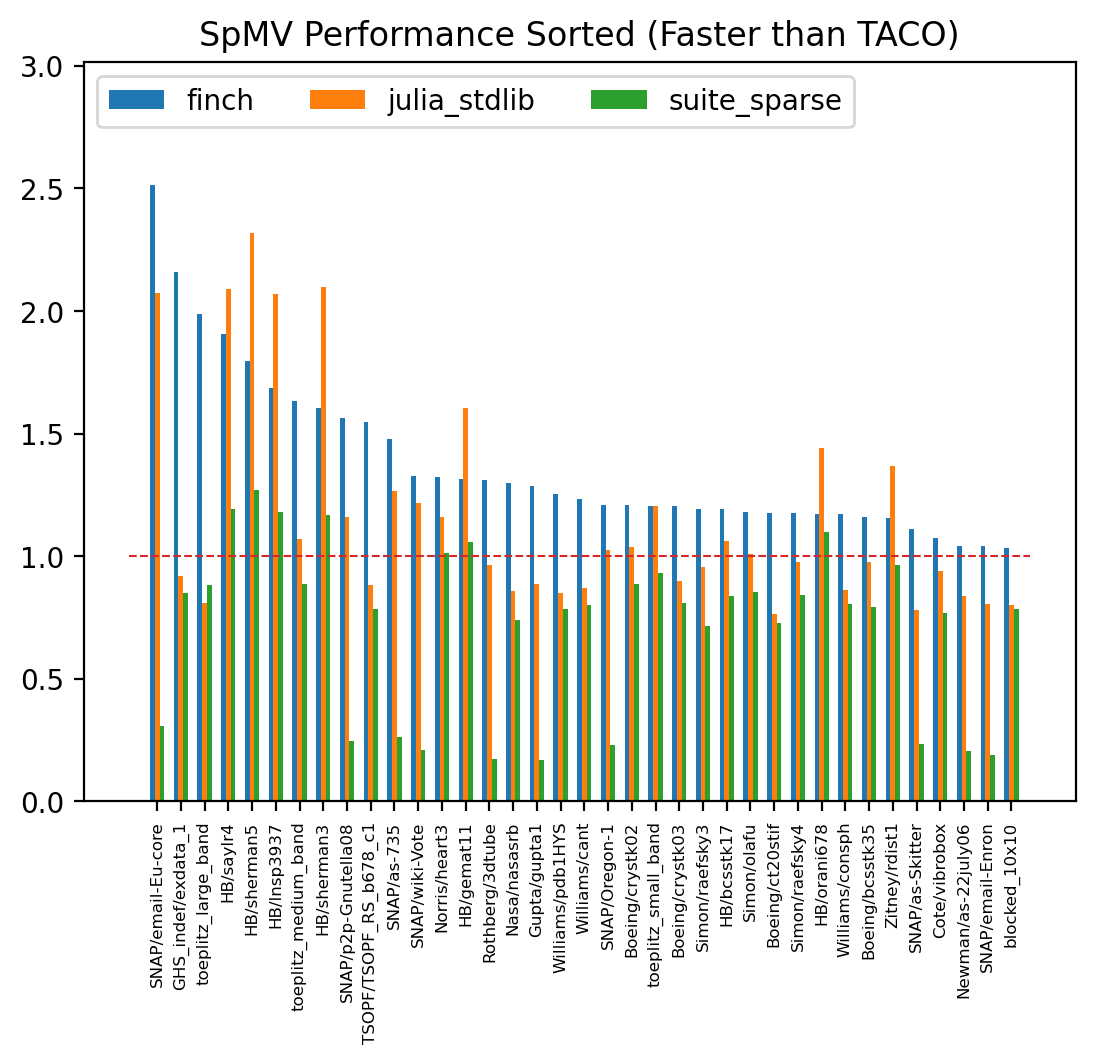
\includegraphics[width=\linewidth]{spmv_performance_sorted_(faster_than_taco).png}
    \end{minipage}%
    \begin{minipage}[t]{0.5\textwidth}
        \vspace{0pt} % Add this to ensure top alignment within minipage
        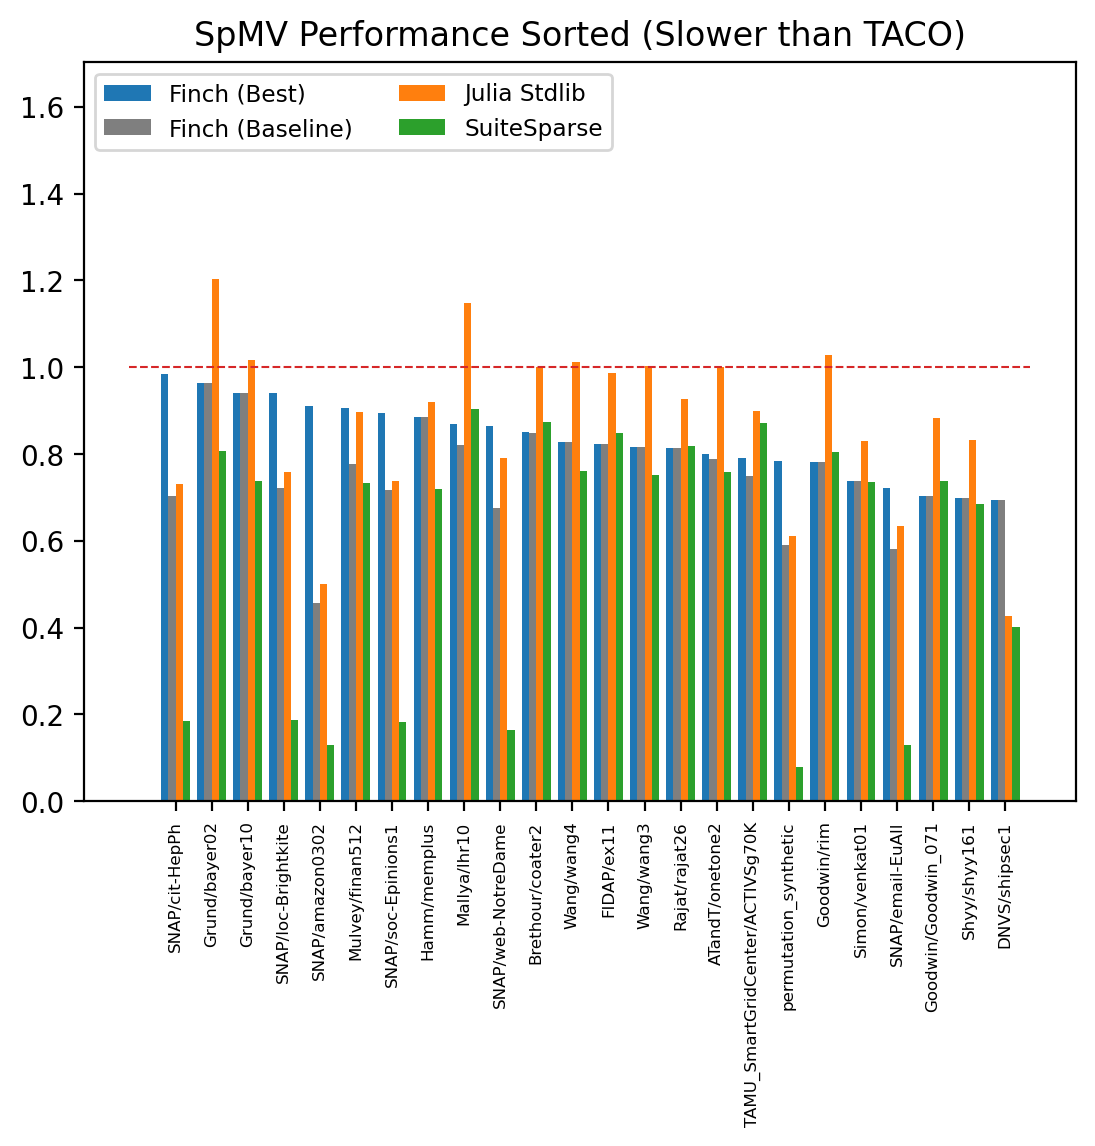
\includegraphics[width=\linewidth]{spmv_performance_sorted_(slower_than_taco).png}
    \end{minipage}
    \caption{Performance of SpMV across various tools.}
\end{figure}

\begin{figure}
    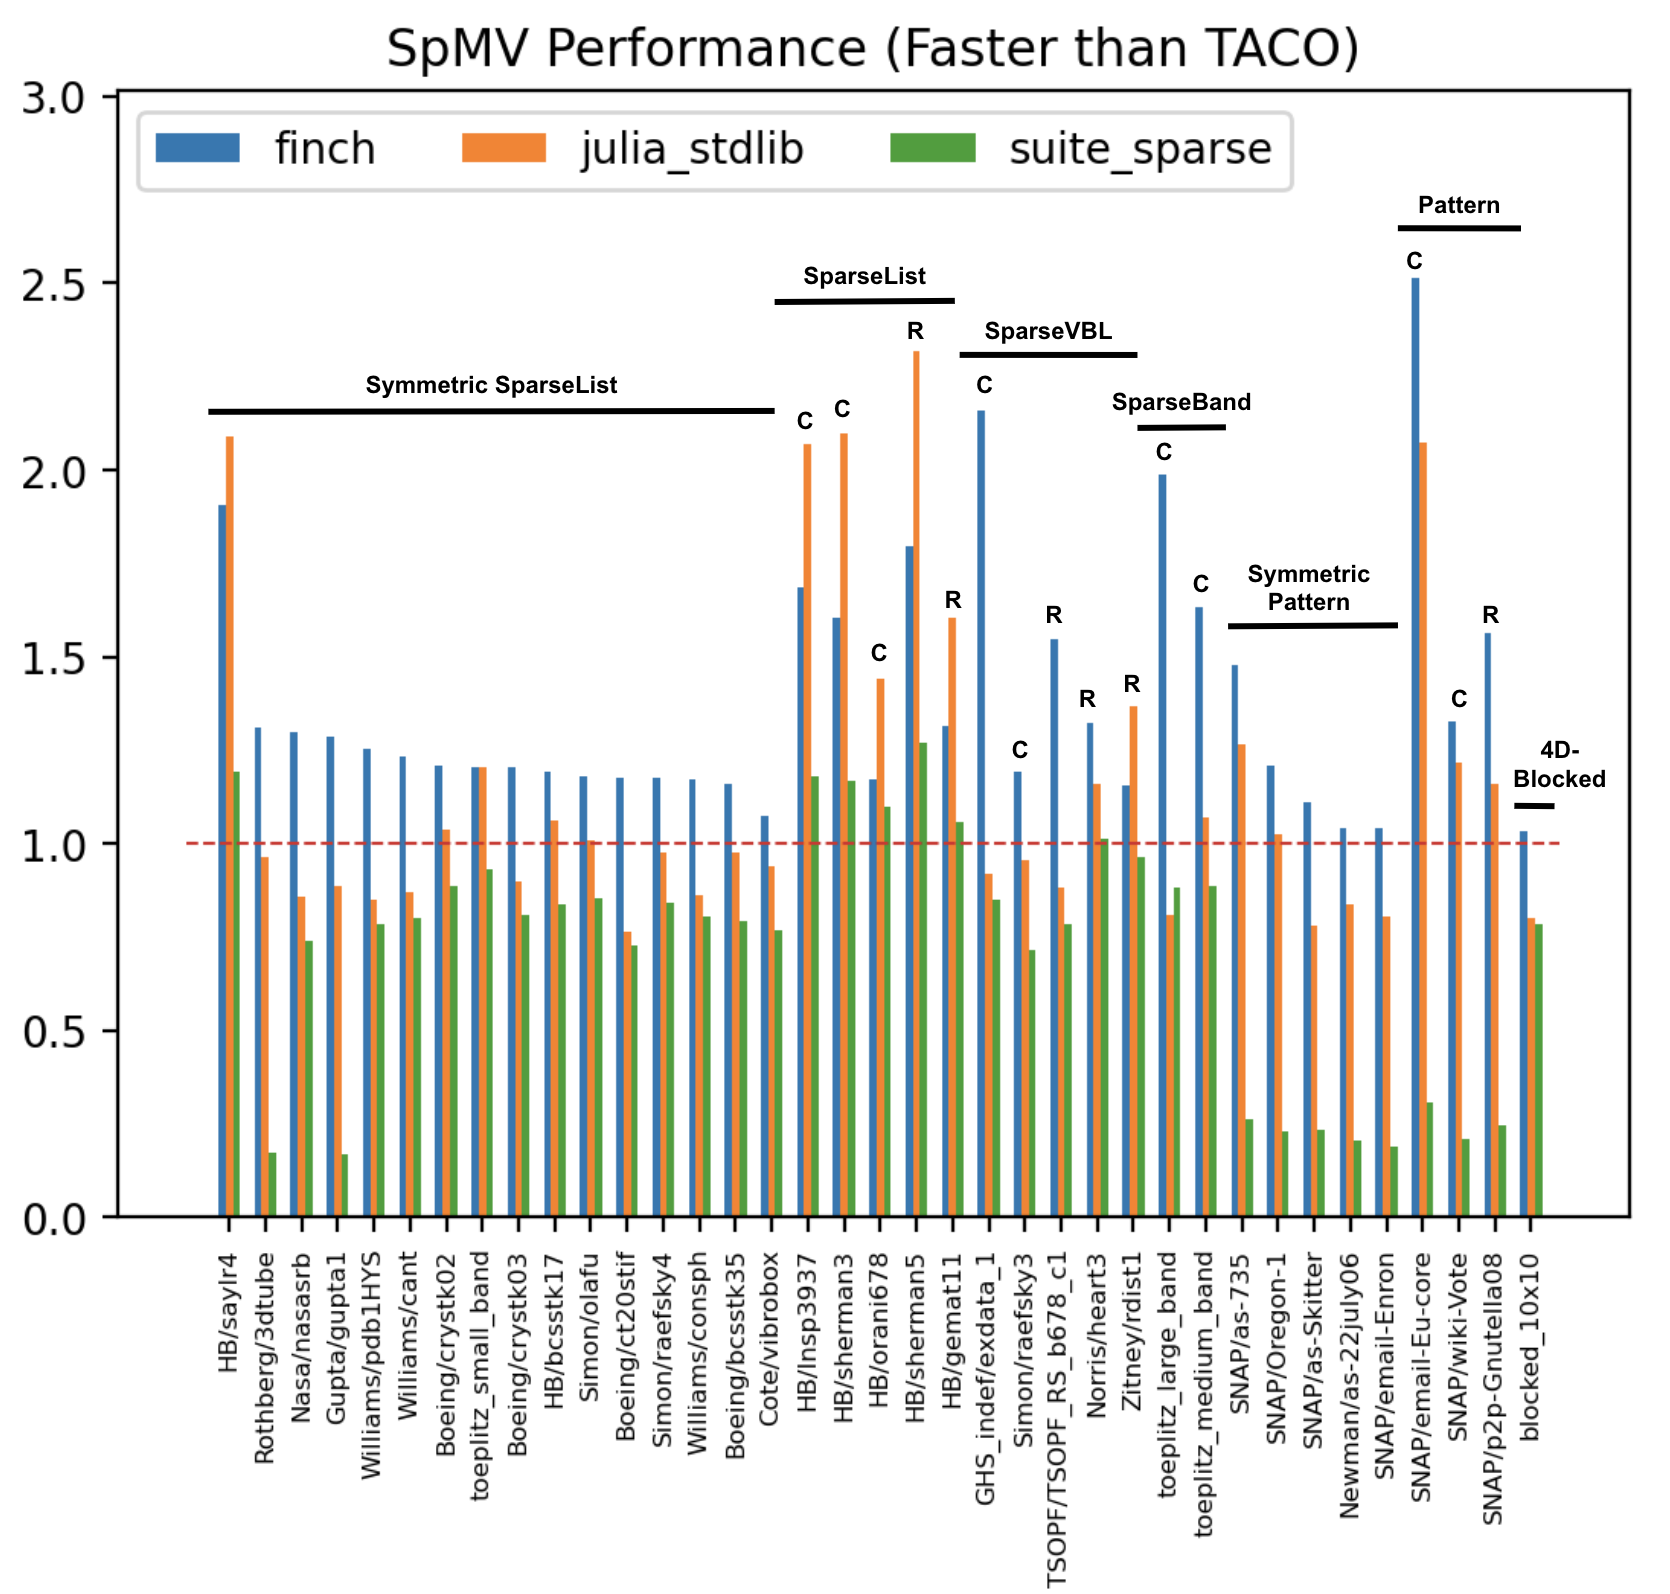
\includegraphics[width=\linewidth]{spmv_performance_grouped.png}
    \caption{Performance of SpMV by Finch format.}
\end{figure}

\subsection{Programming over flexible data}

\subsubsection{Image Morphology}

\help{In this section, explain what erosion is, link a few cool images that show erosion, and then explain what the finch kernel looks like. in particular, be sure to point out that we're doing unrolled convolution, and how that maps to the generated code (merging shifted sparse iterators).}

\help{Explain the role of formats in this kernel, how sparseRLE(PAttern) is really the right thing to use here}

\help{Explain that finch can support a bitwise version, and that finch can mask the bitwise kernel too to get performance with a small change to the code}

\help{Point out that masks with SparseRLE can sometimes perform better because they lift the masking out of the inner loop. Talk about hist and also the fact that Finch supports scatter, here and in spgemm.}

\begin{figure}
	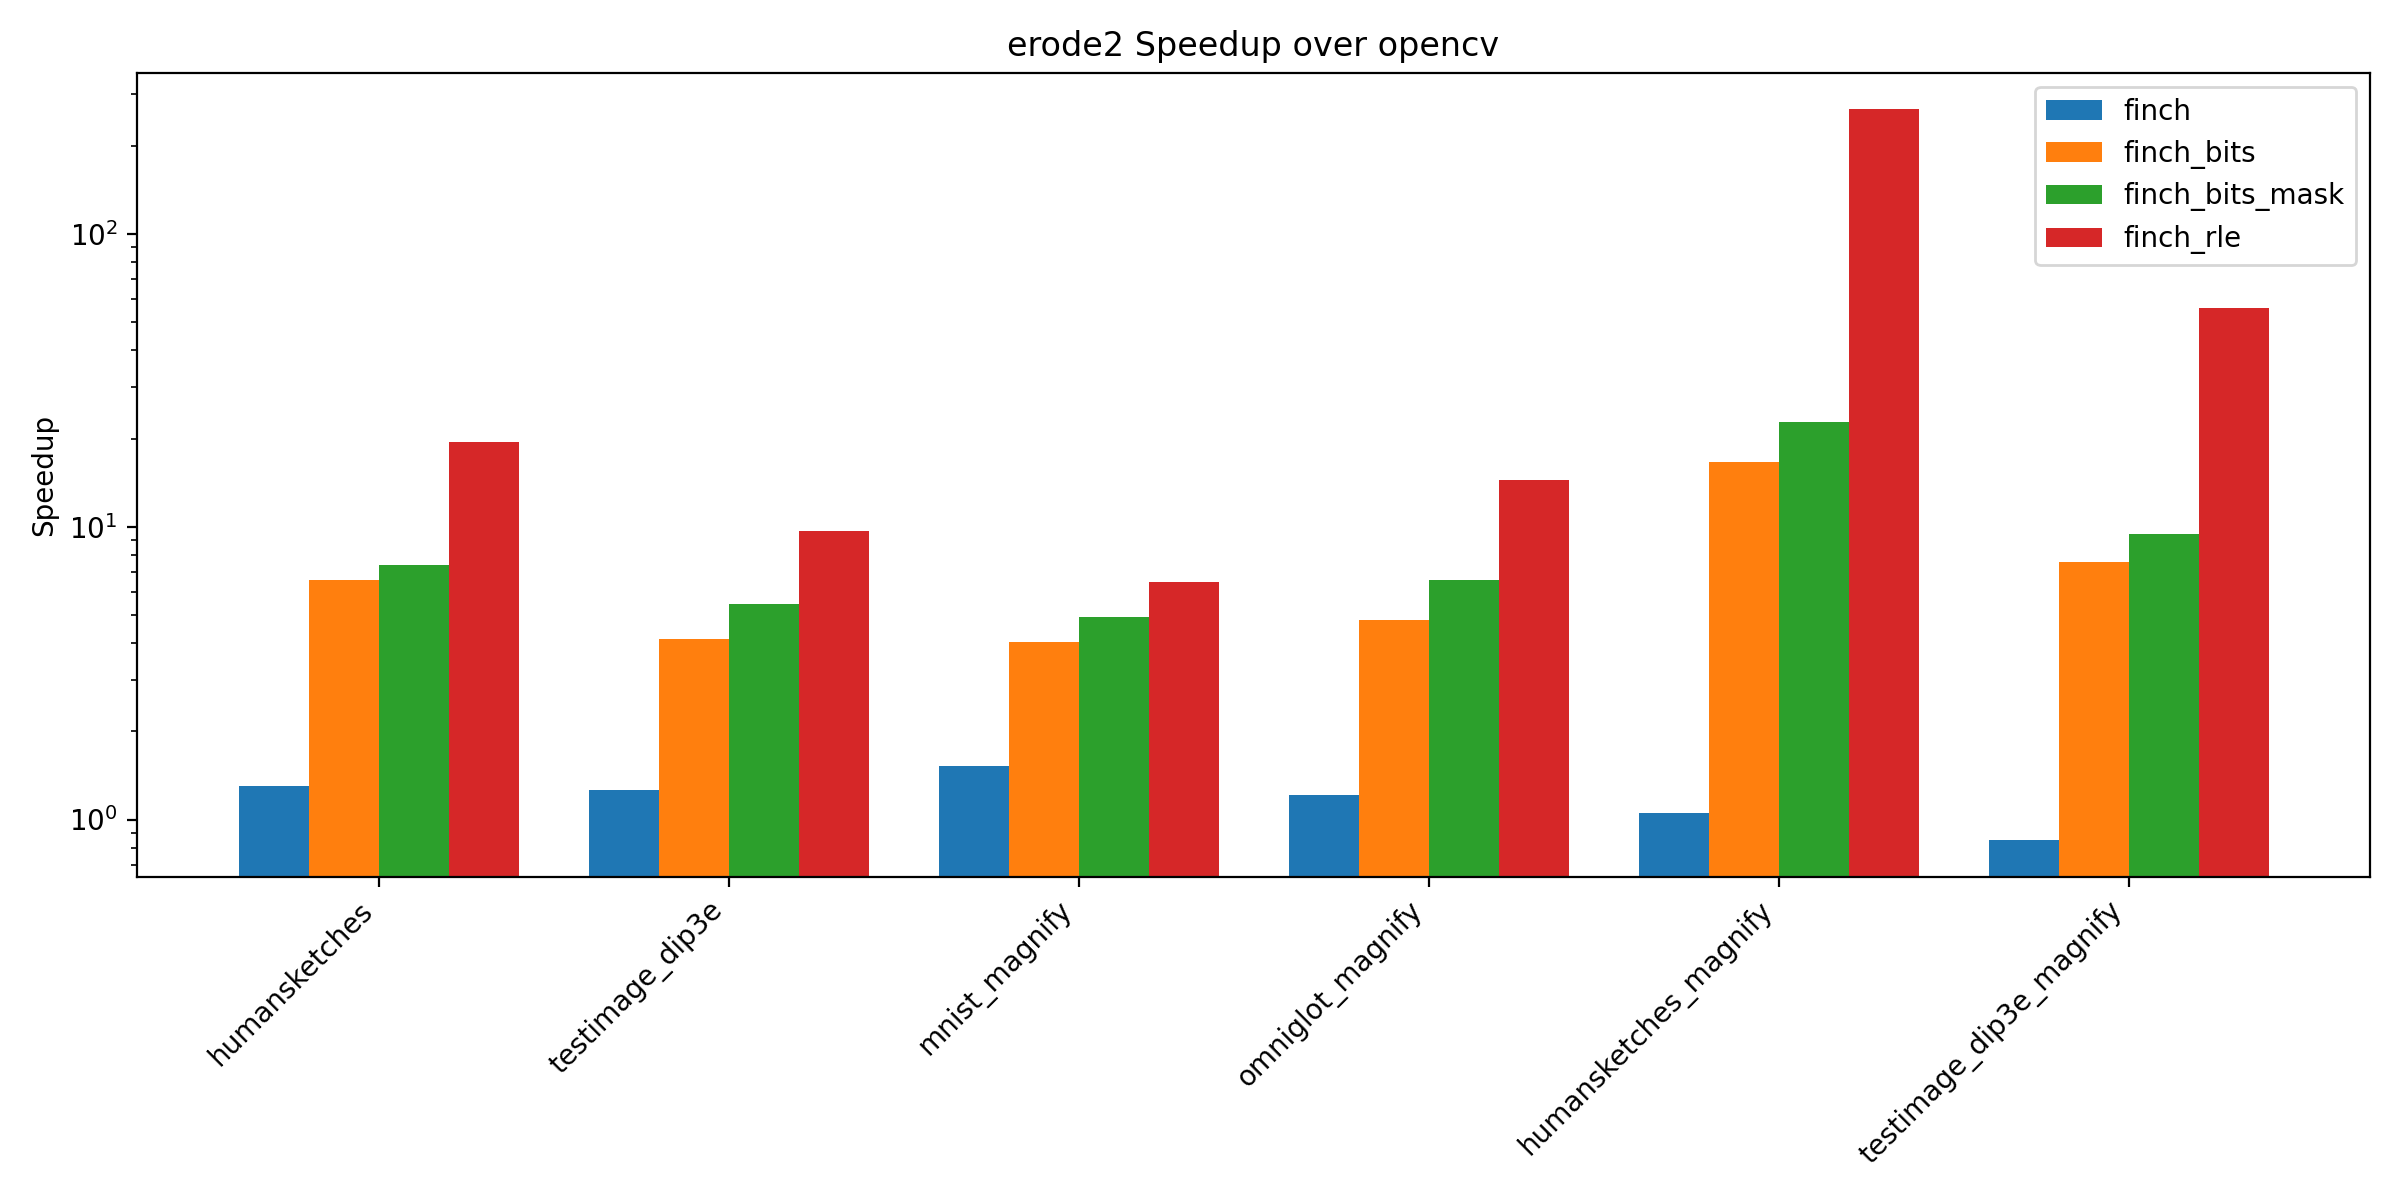
\includegraphics[width=\linewidth]{erode2_speedup_over_opencv.png}
    \caption{Performance of Finch on erosion task (2 iterations).}
\end{figure}

\begin{figure}
	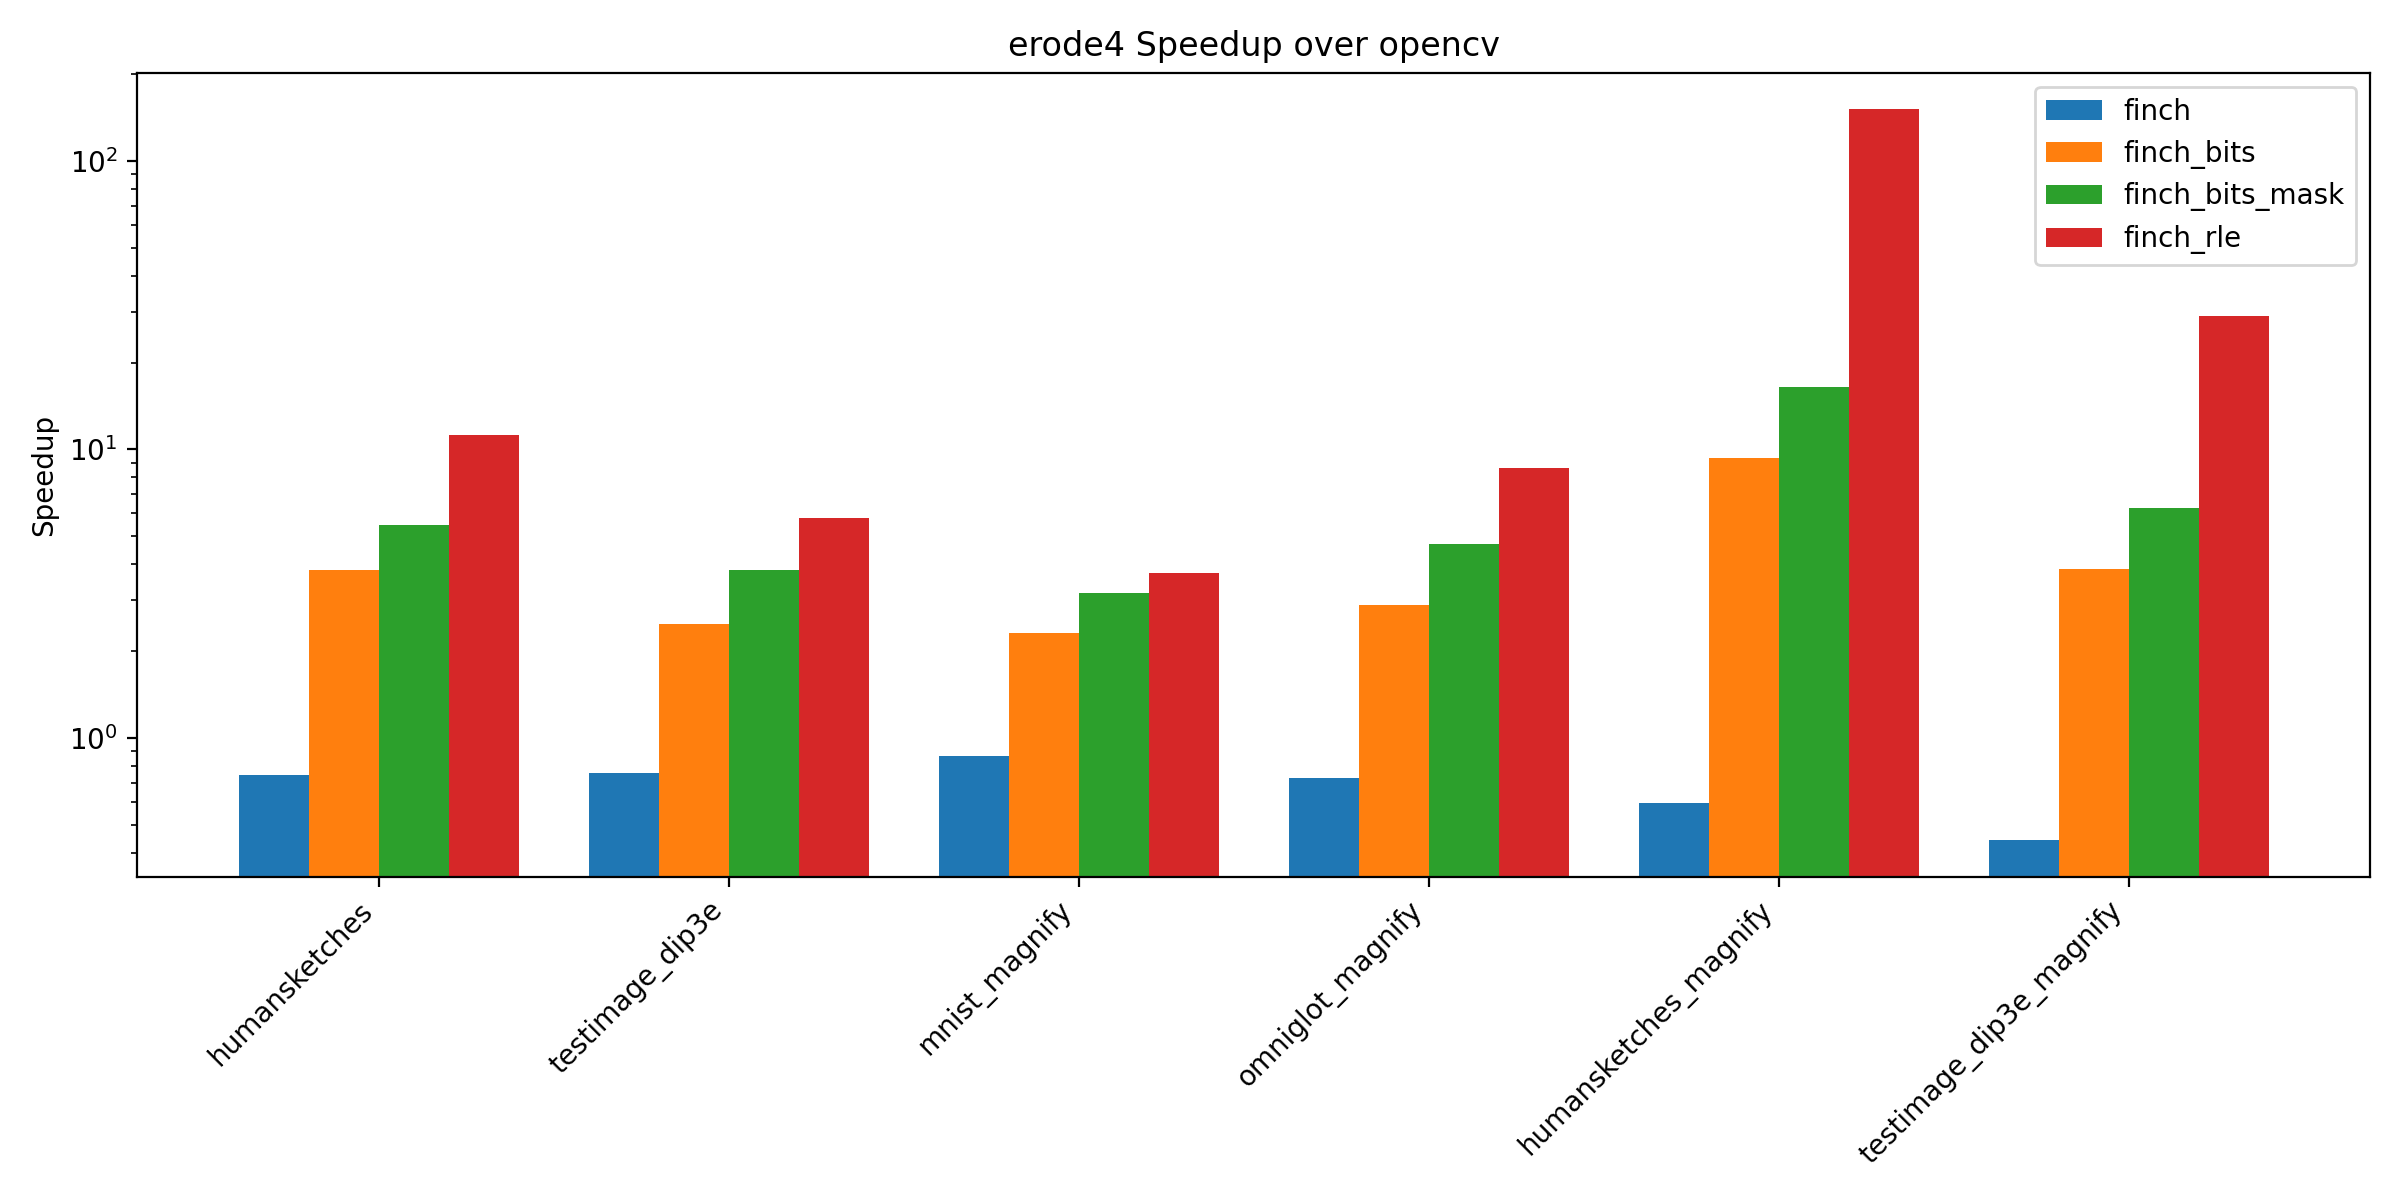
\includegraphics[width=\linewidth]{erode4_speedup_over_opencv.png}
    \caption{Performance of Finch on erosion task (4 iterations).}
\end{figure}

\begin{figure}
	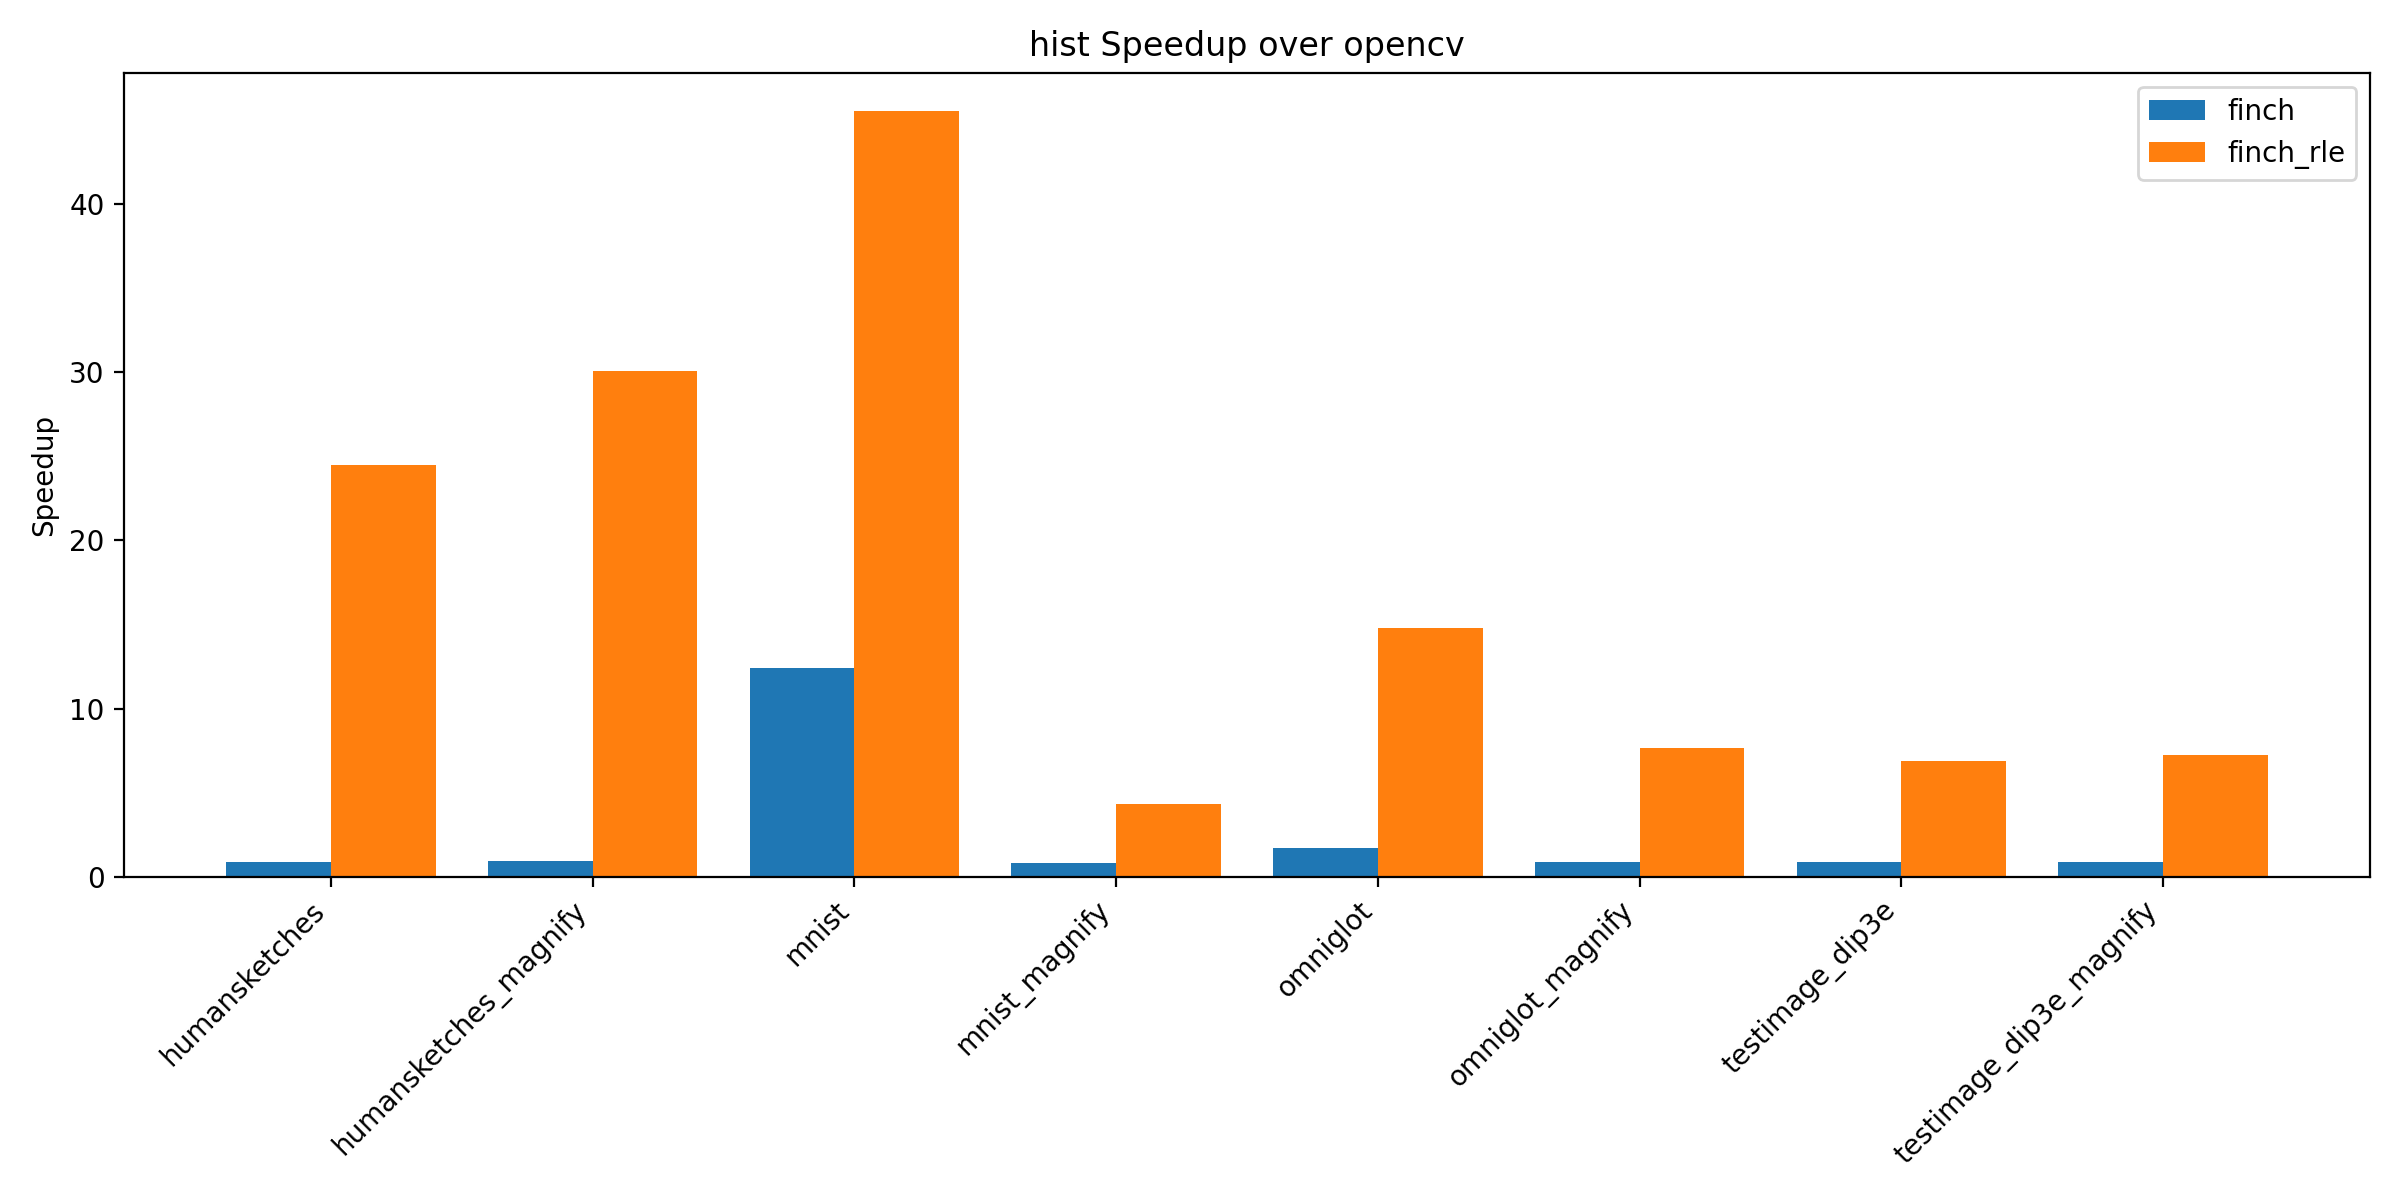
\includegraphics[width=\linewidth]{hist_speedup_over_opencv.png}
    \caption{Performance of Finch on masked histogram task.}
\end{figure}

\subsubsection{Graph Analytics}
\help{In this case, the two main highlights are that Finch can do arbitrary operators (i.e. choose), and that Finch can do early break, and also the different loop orders and multiple outputs. We may need to explain a little bit about what push pull is. For bellman, the main point is that we need multiple outputs, sparse inputs, masks, and sparse outputs with differing formats at differing points.}

\begin{figure}
	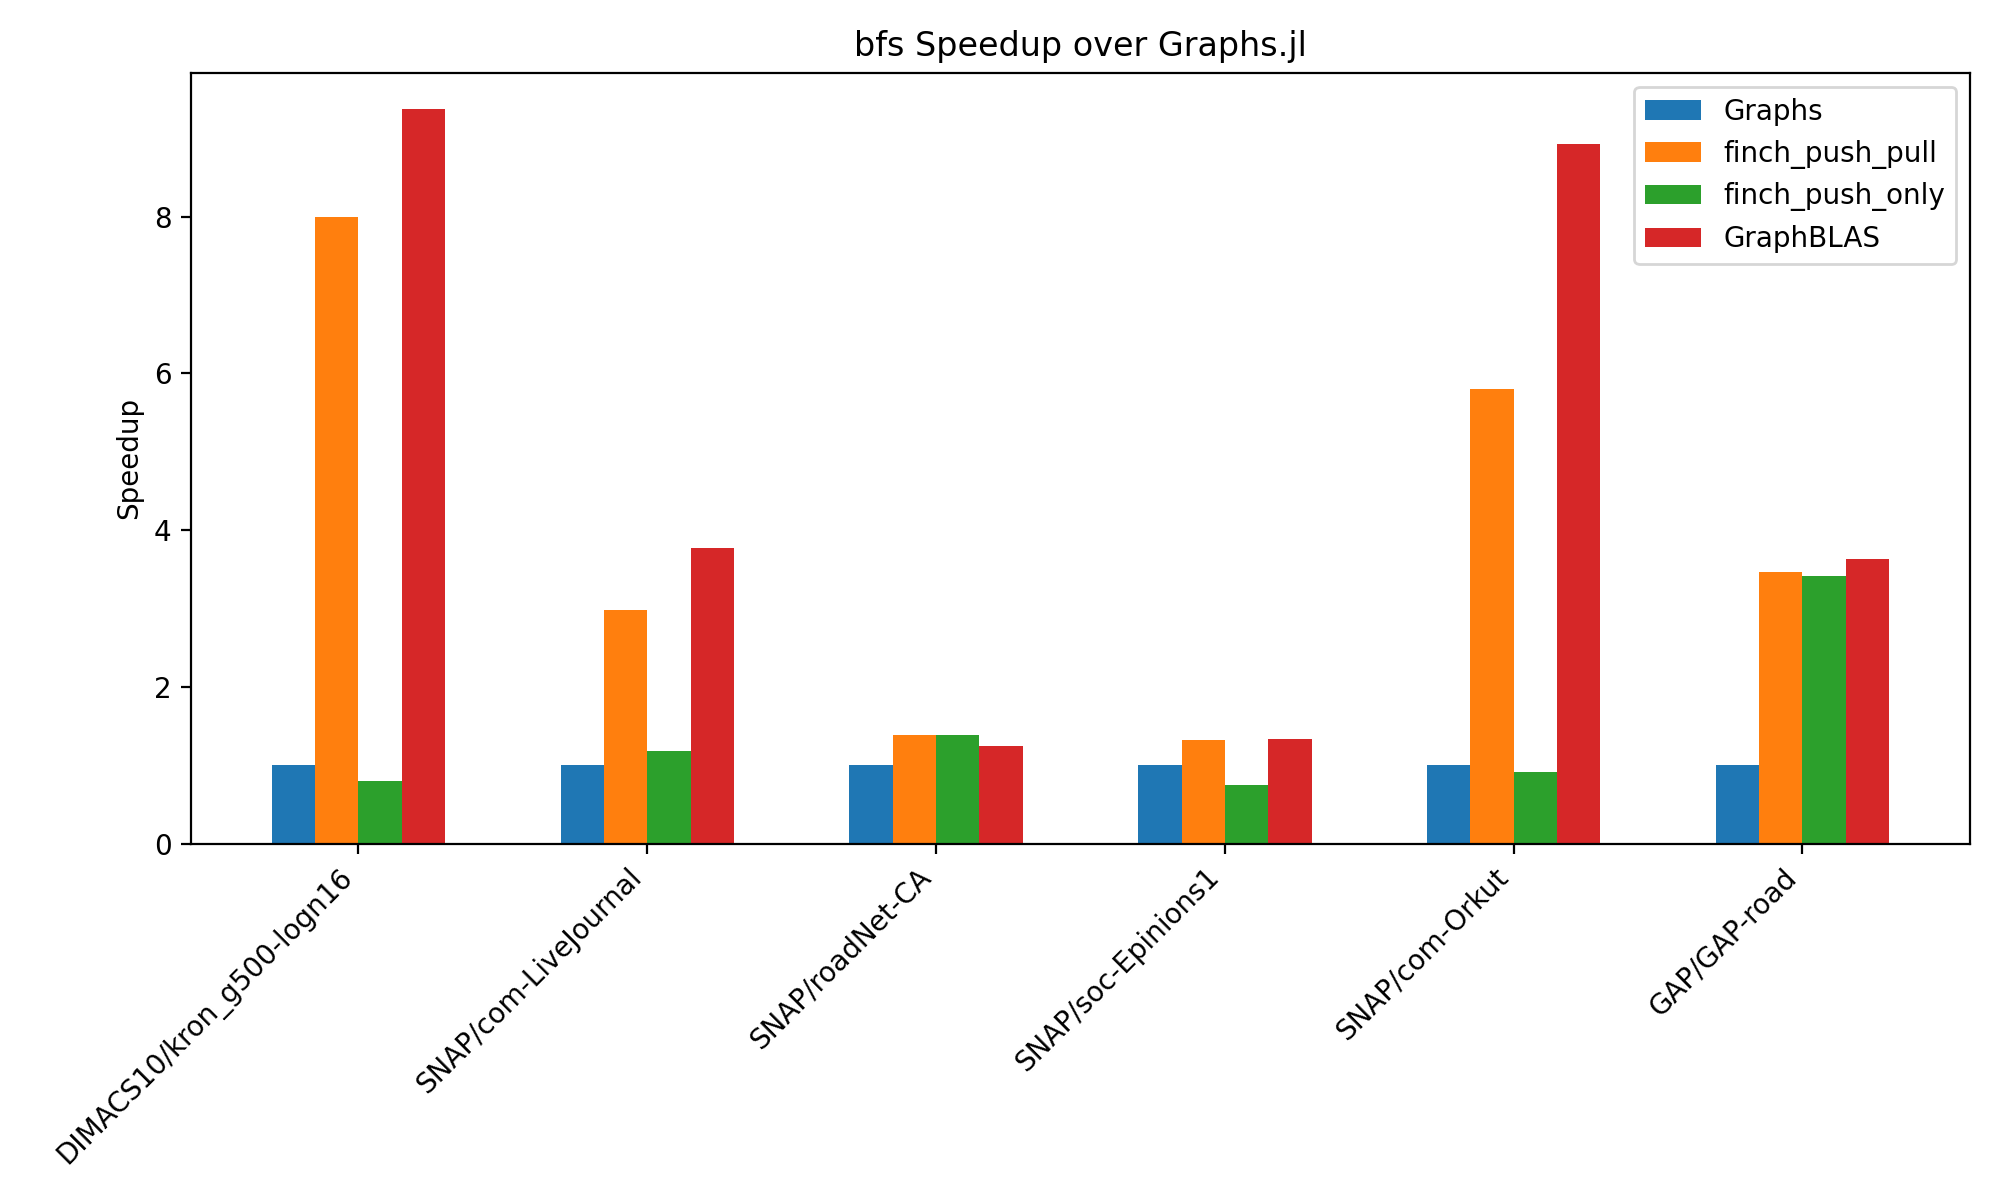
\includegraphics[width=\linewidth]{bfs_speedup_over_graphs.jl.png}
	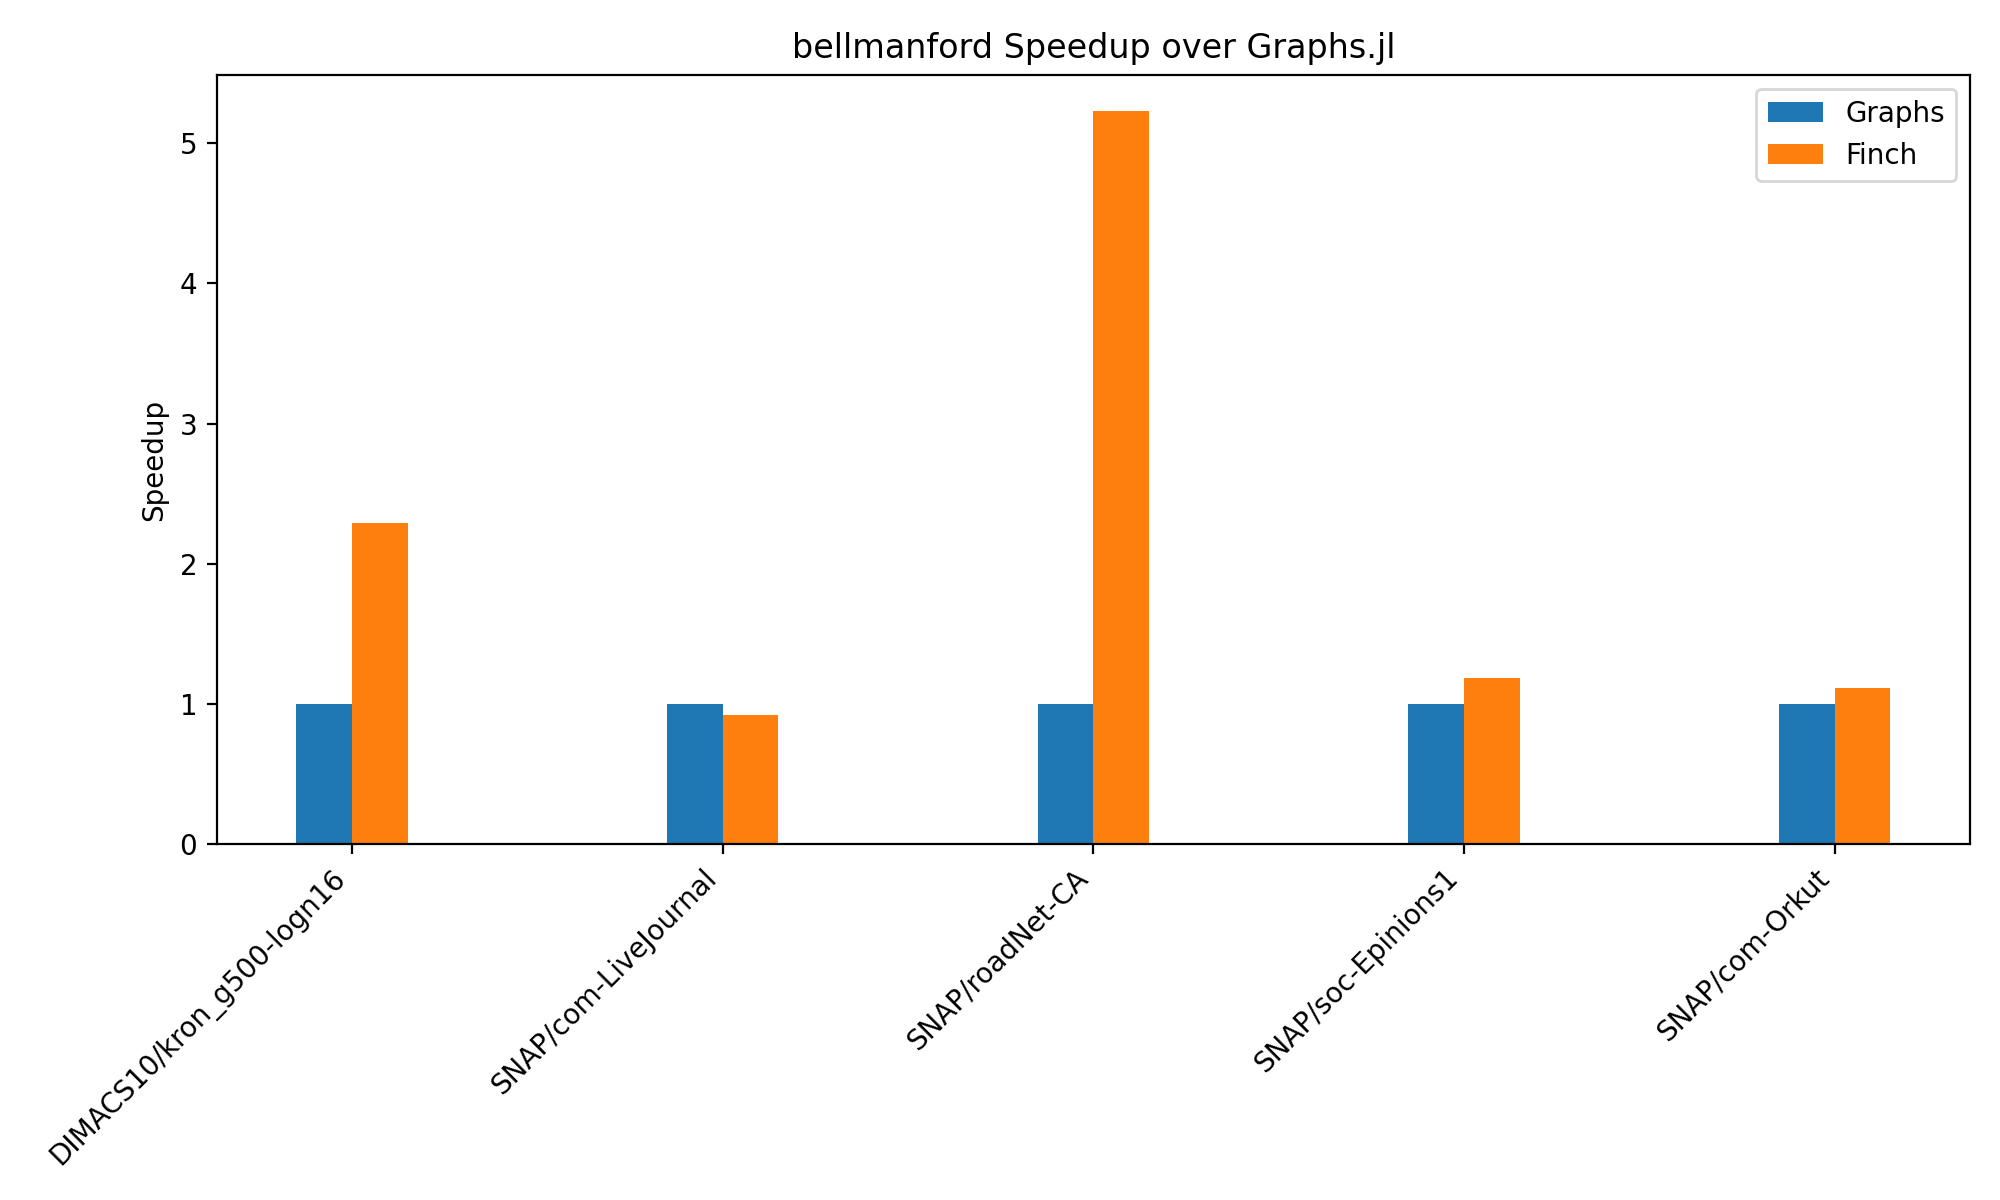
\includegraphics[width=\linewidth]{bellmanford_speedup_over_graphs.jl.png}
    \caption{Performance of graph apps across various tools.}
\end{figure}

Push-Pull BFS in Finch:
\begin{minted}{julia}
V = Tensor(Dense(Element(false)))
P = Tensor(Dense(Element(0)))
F = Tensor(SparseByteMap(Pattern()))
_F = Tensor(SparseByteMap(Pattern()))
A = Tensor(Dense(SparseList(Pattern())))
AT = Tensor(Dense(SparseList(Pattern())))

function finch_bfs_push_kernel(_F, F, A, V, P)
    @finch begin
        _F .= false
        for j=_, k=_
            if F[j] && A[k, j] && !(V[k])
                _F[k] |= true
                P[k] <<choose(0)>>= j #Only set the parent for this vertex
            end
        end
        return _F
    end
end


function finch_bfs_pull_kernel(_F, F, AT, V, P)
    p = ShortCircuitScalar{0}()
    @finch begin
        _F .= false
        for k=_
            if !V[k]
                p .= 0
                for j=_
                    if F[follow(j)] && AT[j, k]
                        p[] <<choose(0)>>= j #Only set the parent for this vertex
                    end
                end
                if p[] != 0
                    _F[k] |= true
                    P[k] = p[]
                end
            end
        end
        return _F
    end
end
\end{minted}

\subsection{Implementing Numpy Array API in Finch}
Experiments:
- elementwise op of 3 things (fused, unfused, julia broadcast, duckdb)
- Matrix multiply (with the insert indices)
- Triangle Counting
- SDDMM




\subsubsection{The Finch High-Level API (Needs a Name)}

\subsubsection{Finch Logic}

\subsubsection{Finch Interpreter}

\subsubsection{Lowering}
\subsubsection{Heuristic Optimization}

Find an example where fusing the python interface gives a big speedup over non-fused kernels.

%matmul, mttkrp, repeated ttm, triangle counting, multiple pointwise,
%in-place.
%dot((v^t .* u), w)) vs. 
%(v^t .* dot(u, w))

%%
%% The acknowledgments section is defined using the "acks" environment
%% (and NOT an unnumbered section). This ensures the proper
%% identification of the section in the article metadata, and the
%% consistent spelling of the heading.
\begin{acks}
    To Mateusz, Hameer, and Jaeyeon for their excellent programming contributions to the Finch codebase.
\end{acks}

%%
%% The next two lines define the bibliography style to be used, and
%% the bibliography file.
\bibliographystyle{ACM-Reference-Format}
\bibliography{FinchOOPSLA.bib, FinchOOPSLAOverleaf.bib}


%%
%% If your work has an appendix, this is the place to put it.
\appendix

\section Frequently Requested Finch kernels 

\end{document}
\endinput